%%%%%%%%%%%%%%%%%%%%%%%%%%%%%%%%%%%%%%%%%%%%%%%%%%%%%%%%%%%%%%%%%%% 
%                                                                 %
%                            ROOT FILE                            %
%                                                                 %
%%%%%%%%%%%%%%%%%%%%%%%%%%%%%%%%%%%%%%%%%%%%%%%%%%%%%%%%%%%%%%%%%%% 
%
%  Run LaTeX or pdfLaTeX on this file to produce your thesis.
%  To produce the abstract title page followed by the abstract,
%  see the file abstitle-phd.tex or abstitle-mas.tex.
%
%%%%%%%%%%%%%%%%%%%%%%%%%%%%%%%%%%%%%%%%%%%%%%%%%%%%%%%%%%%%%%%%%%%

\documentclass[chap]{thesis}

% Use the first command below if you want captions over 1 line indented. A side
% effect of this is to remove the use of bold for captions (thesis default).
% To restore bold, also include the second line below.
\usepackage[hang]{caption}      % to indent subsequent lines of captions
\usepackage{makeidx}
\usepackage{amsmath}
\usepackage{ amssymb }
\usepackage{graphicx}
\usepackage{algorithm2e}
\newcommand{\tuple}[2] {\langle #1,#2\rangle}
\renewcommand{\captionfont}{\bfseries} % bold caption (needed with caption 
                                       % package to restore boldface.)
\newtheorem{principle}{Principle}
\newtheorem{definition}{Definition}
\newtheorem{theorem}{Theorem}
\newtheorem{proposition}{Proposition}
\newtheorem{corollary}{Corollary}
%\includeonly{rpichap1}  % use \includeonly to process only
                         % the file(s) listed inside the braces                       
\begin{document}
 
%%%%%%%%%%%%%%%%%%%%%%%%%%%%%%%%%%%%%%%%%%%%%%%%%%%%%%%%%%%%%%%%%%% 
%                                                                 %
%                            TITLE PAGE                           %
%               Master's Thesis or Master's Project               %
%                                                                 %
%%%%%%%%%%%%%%%%%%%%%%%%%%%%%%%%%%%%%%%%%%%%%%%%%%%%%%%%%%%%%%%%%%% 
%  This file produces the title page, copyright page (if requested)
%  and the Table of Contents, List of Figures and List of Tables.
% 
%  To produce the abstract title page followed by the abstract,
%  see the template file, "abstitle-mas.tex"
%%%%%%%%%%%%%%%%%%%%%%%%%%%%%%%%%%%%%%%%%%%%%%%%%%%%%%%%%%%%%%%%%%%

% Supply information for use on title page:    
\thesistitle{\bf Extended Balance Theory\\ and Convergence Model\\in Social Networks}        
\author{Yi Qian}        
\degree{Master of Science} 
\department{Computer Science} % provide your area of study here; e.g.,
%  "Mechanical Engineering", "Nuclear Engineering", "Physics", etc.      
\signaturelines{3}
\projadviser{Sibel Adal\i} % For a masters project use \projadviser instead of \thadviser,
\memberone{Elliot Enshelevich}        
\membertwo{Petros Drineas}
%\memberthree{Aristotle} % must change signaturelines to 4 if using this 4 members
%\projadviser {Sibel Adal\i, Elliot Enshelevich, Petros Drineas}
%\cocoprojadviser{Elliot Enshelevich, Petros Drineas} %if needed
%\cocothadviser{Second co-adviser} % if needed
%  For a masters project use \projadviser instead of \thadviser, 
%  and \coprojadviser and \cocoprojadviser if needed.    
\submitdate{March 2013\\(For Graduation May 2013)}        
\copyrightyear{2013}   % if omitted, current year is used.        

% Print titlepage and other prefatory material:   
\titlepage     
\copyrightpage         %optional           
\tableofcontents        
\listoftables          %required if there are tables
\listoffigures         %required if there are figures

   % titlepage material for Master's thesis or project
%\include{rpititle-phd}   % titlepage material for PhD thesis 
%%%%%%%%%%%%%%%%%%%%%%%%%%%%%%%%%%%%%%%%%%%%%%%%%%%%%%%%%%%%%%%%%%% 
%                                                                 %
%                         ACKNOWLEDGEMENT                         %
%                                                                 %
%%%%%%%%%%%%%%%%%%%%%%%%%%%%%%%%%%%%%%%%%%%%%%%%%%%%%%%%%%%%%%%%%%% 
 
\specialhead{ACKNOWLEDGMENT}
 It has been a great privilege to spend two and a half years in the Department of Computer Science at Rensselaer Polytechnic Institute. One of the joys of a completion is to look over the journey past and remember all the people who have helped and supported me along this long but fulfilling road.
 
 My first debt of gratitude must go to my advisor, Dr. Sibel Adal\i. She patiently provided the vision, encouragement and advise necessary for me to proceed the research journey. I hope that I could be as lively, enthusiastic, and energetic as 
Sibel and to someday be able to command an audience as well as she can. Not only that she has always been an inspirational and experienced advisor to me throughout my graduate school years, but also she supports my choice in exploring various subjects with great freedom. I could not have asked for a better role model as a researcher, as well as a great person.


I would like to thank my committee, Dr. Elliot Anshelevich and Dr. Petros Drineas for their support and guidance. Special thanks to Dr. Elliot Anshelevich to his many valuable suggestions. The guidance has served me well and I owe them my heartfelt appreciation.
 
I wish to thank my parents, Guahua Qian and Pinhong Jiang. Their love provided my inspiration and was my driving force through the years. My girl, Feifei Bian, whose love and encouragement brings me all the way here. In our four-year relationship, we bear the brunt of frustration and share the joy of success.  Without the love and support of them, I would certainly not be able to finish this thesis.

I also would like to thank T. DuBois for sharing the implementation details of his algorithm.

%%%%%%%%%%%%%%%%%%%%%%%%%%%%%%%%%%%%%%%%%%%%%%%%%%%%%%%%%%%%%%%%%%% 
%                                                                 %
%                            ABSTRACT                             %
%                                                                 %
%%%%%%%%%%%%%%%%%%%%%%%%%%%%%%%%%%%%%%%%%%%%%%%%%%%%%%%%%%%%%%%%%%% 
 
\specialhead{ABSTRACT}

Structural balance theory studies the influence between positive and negative relationships in a social network. Researchers regard structural balance as a sound and universal concept in social networks. We first observe the fact that current structural balance theory does not distinguish between varying strengths of relationships, which is shown to be of good significance in many social interactions. We address this problem by analyzing the social and psychological source of imbalance, and establish an extended theory that defines balance in networks with varying relationship strengths.  We show how balance is reasoned when strengths of relationships are measured by either a totally ordered set, or by numerical values. Our extended balance theory is shown to be a generalization of the current structural balance theory.

The convergence model studies how an imbalanced network evolves towards new balance. The assumption behind our model of convergence is that in resolving tensions within imbalanced relationships, people tend to avoid the effort involved in changing relationships if possible. The introduction of extended balance theory allows us to formulate the convergence problem of a social network as a Metric Multidimensional Scaling (MDS) optimization problem. 

Modeling the dynamic nature of social networks, the convergence model inherits a predictive power on unknown relationships. We show that a list of famous social network phenomena, such as ``If two people have more common friends, then they are more likely to become friends", hold under the convergence model. Moreover, we use the convergence model to study the {\it edge sign prediction problem}. In a social network with positive and negative signed edges, the task of sign prediction is to infer the signs of a small fraction of ``hidden" edges based on the information from the rest of the network. We show why and how the convergence model can be applied in prediction tasks over real online social network datasets. Stress majorization technique is used to compute the convergence, and our method consistently matches and outperforms the state of art.

%1. The motivation of an extended balance theory with relations of strengths.
%2. Address the balance tendency assumption. 
%The possible applications of balance tendency (convergence), and the unsolved problems. 
%3. Propose signed edge prediction as an application of social network convergence.
%4. Outline the structure of the thesis

%%%%%%%%%%%%%%%%%%%%%%%%%%%%%%%%%%%%%%%%%%%%%%%%%%%%%%%%%%%%%%%%%%% 
%                                                                 %
%                            CHAPTER ONE                          %
%                                                                 %
%%%%%%%%%%%%%%%%%%%%%%%%%%%%%%%%%%%%%%%%%%%%%%%%%%%%%%%%%%%%%%%%%%% 
 
\chapter{INTRODUCTION}
In a social network with signed edges, positive edges
represent friendship while negative edges represent antagonism. An important problem
in the study of social networks is to understand the tension between these two forces~\cite{kleinberg-book}. Structural balance is a concept studying the influence of signed relationships on each other. The theory of structural balance has its origins in the work of Heider~\cite{Heider:46}. Cartwright and Harary then formalized Heider's idea and formulated the overall structure of a network with signed edges~\cite{Cartwright:56}. Davis~\cite{Davis:67} further gives a generalized theory by a relaxed balance assumption. In essence, structural balance theory considers certain configurations of positive and negative edges as socially and psychologically more plausible than others. In balance theory, a triangle, i.e. triad, is the smallest structural unit. It consists of three pairwise relationships between three people, and there are four distinct ways to label each relationship as positive or negative; see Figure~\ref{fig:balance_strong}
\begin{figure}[th]
\centering
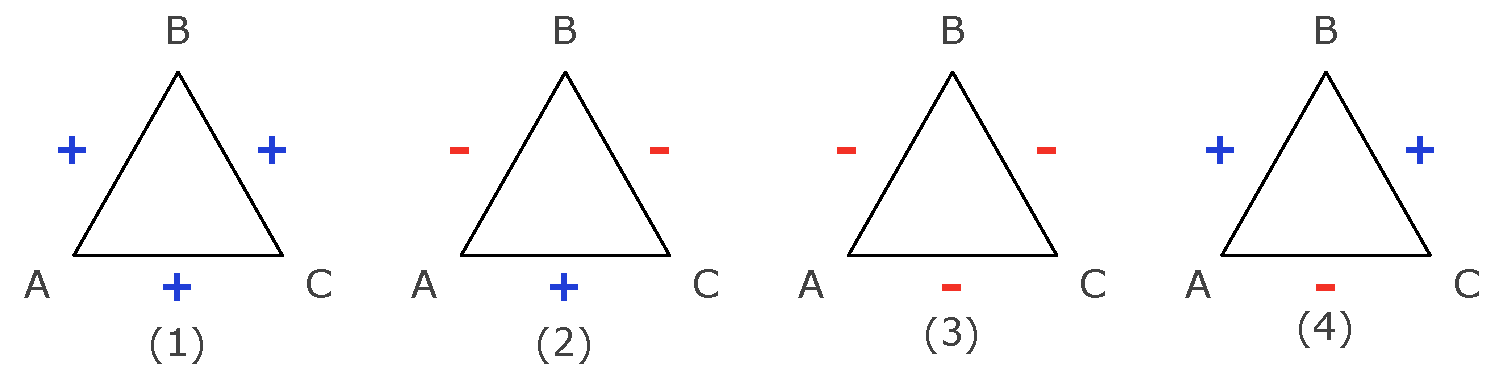
\includegraphics[width=4.8in]{Figs/strongBalance_hor.pdf}
\caption{\label{fig:balance_strong} Four different cases of triangular relationship.}
\end{figure}\\
It is argued that triads (1) (2) are more socially and psychologically reasonable than than triads (3) and (4)~\cite{Heider:46},~\cite{Cartwright:56}. The configurations of positive and negative relations in triads (3) (4) will bring tension that makes such triadic relationship unstable. Davis points out that the stress inside triad (4) is much more significant than it is in triad (3), and hence proposes a generalized balance theorem~\cite{Davis:67}. 

The structural balance theory provides a concise and elegant description of influence between interpersonal relationships. Moreover, it illustrates a nice connection between local configuration and global structural property in social networks. The key result of Cartwright-Harary's work is the structure theorem~\cite{Cartwright:56}: if a network is balanced, the nodes can be partitioned into two subsets such that all positive relationships are within subsets and all negative relationships are between subsets. Davis draws a similar theorem in the case when triad (3) in Figure~\ref{fig:balance_strong} is relaxed as balanced~\cite{Davis:67}. 

In recent research in online social networks, network balance plays a key role in many applications. One specific problem of interest is inferring new relationships and make recommendations based on existing relationships. We observe that the concept of structural balance is widely applied when developing algorithms for this type of prediction task. For example, Leskovec et al. generate a class of �triad features� in their prediction algorithm, i.e. a pair of relationships constraining a third relationship~\cite{Leskovec:2010}. They also use the structural balance as a touchstone to see the congruence between their practical results and the long studied theory. Another algorithm~\cite{golbeck:distrust2011} makes use of similar assumptions without explicit mention of balance theory in which trust and distrust relationships are mapped to metric distances on a continuous range. To some degree, the strong prediction performance of these algorithms justifies the structural balance theory. However, we will see the theory has its own weakness.
 
The arguments behind the balance theory imply a type of tendency towards balance for general social networks. That is, every social network will evolve to a state where every triad in it is balanced. The assumption by itself is congruent and intuitive; unstable triadic relationships (triads (3) (4) in Figure~\ref{fig:balance_strong}) will break and change to stable ones because of the inside tension. Regardless of other potential factors, a social network will inevitably reach a balanced state. As the ``balance process" is by nature a convergent process, every social network is expected to stay at a largely structurally balanced state. However, for most observed signed structures for social groups, exact structural balance does not hold~\cite{Doreian:02}. 

Despite the fact the structural balance theory is insufficient of empirical support, we regard the balance tendency a sound and natural description of social networks. In the physical world, an object stays at a state of minimum energy. Analogically, in social networks, does a triadic relationship stays at a state with minimum inner tension? We regard the structural balance theory as an incomplete description of balance in social networks. The current theory only deals with binary relationships while relationships in practice vary in degrees. While it is shown that strength is an important factor in many different social phenomena~\cite{Granovetter:1973}, the structural balance theory does not distinguish between relationships of the same sign but different strengths. In fact, when Cartwright and Harary first formalized the theory of structural balance, they also had the  following suggestions \cite{Cartwright:56}:

{\it ``...Obviously, however, many relationships of interest to psychologists(like liking, for example) exist in varying degrees. The fact means that our present use of graph theory can treat only the structural, and not the numerical, aspects of relations. While our treatment is thereby an incomplete representation of the strength of relations, we believe that conceptualization of the structural properties of relations is a necessary first step toward a more adequate treatment of the more complex situation." }

We take steps to analyze the social and psychological source of imbalance, and propose two fundamental principles regarding triadic balance in the general sense. Based on the principles, we establish an extended balance theory that deals with relationships with varying strengths. Heider's structural balance theory will be shown to be a special case under the generalized theory. 

In the second part of the thesis, we study the problem of social network convergence. The balance theory defines what is a  balanced state of a social network, but does not describe the dynamic aspect of the ``balance process". The problems of what each imbalanced triad will change to over time, and globally how an imbalanced network would evolve towards balance has not been studied in literature. It is plausible to have a decisive argument on whether triad (4) in Figure~\ref{fig:balance_strong} will change to triad (1) or triad (2), given the imperfect empirical evidence of structural balance itself. That is, if Bob's two friends Alice and Chris cannot get along with each other, whether Alice and Chris will resolve conflicts and become friends, or Bob teams up with one of them? In real life, questions like this really depend on how close Bob and Alice (Chris) is and how much conflict there is between Alice and Chris. For example, if the two friendships are very close while the conflict is subtle, we expect to see Alice and Chris become friends. On the contrary, if Bob is only close to Alice while the hatred between Alice and Chris is intense, it is likely that Bob will team up with Alice. With the extended balance theory, the problem becomes non-trivial and potentially solvable. We call such dynamic ``balance process" the {\bf social network convergence}. 

The convergence model helps complete the ``process" of network balance, as it models the principles of inter-relationship influence aspect of the network evolution. Due to its dynamic nature, the convergence model should inherit a predictive power over new relationships. For example, the strong triadic closure states that two people with a common close friend are very likely to friend each other in the future~\cite{Granovetter:1973}. We propose some famous predictive properties in social networks, such as ``two people with more common friends are more likely to become friends" as touchstones of the model, and show they hold under the convergence model. Both empirical experimental results and proofs are given.

To further justify our theory empirically, we use the convergence model to study the {\it edge sign prediction} problem. The {\it edge sign prediction} problem uses information of existing relationships to infer hidden relationships. To this date, many algorithms for this prediction problem are based on machine learning methods. These methods generate multiple structural features from the known relationships, and then use these features to classify the unknown relationships~\cite{Leskovec:2010},~\cite{golbeck:distrust2011},\cite{Guha:04}. We show why and how the convergence model can be applied in the prediction tasks over real online social network datasets. Our method consistently matches and outperforms the state of the art.

To summarize, we make the following
unique contributions in this thesis:
\begin{itemize}
\item We first introduce a new extended balance theory that allows
  arbitrary relationship strengths. We express balance with two
  simple principles that preserve the unique meaning of a
  positive, and a negative
  relationship. We show how balance can be reasoned when the strength of
  relationships are expressed as either discrete categorical values,
  as pairwise comparisons or as metric distances using the same two
  principles. Our method is novel, has sound social and psychological
  basis and captures the classical balance theory as a special case.
\item We propose a convergence model, describing how an imbalanced
  network evolves towards new balance. The assumption behind our model
  is that in resolving tensions within imbalanced relationships,
  people tend to avoid the effort of changing relationships if
  possible. The introduction of extended balance theory allows us to
  formulate the convergence problem of a social network as a Metric
  Multidimensional Scaling (MDS) optimization problem.
\item We show how the convergence model can be used to predict edge
  signs in social networks, and justify our theory through experiments
  on real datasets. Stress majorization is applied to solve
  MDS~\cite{Gansner:05}, and our method consistently matches and
  outperforms the state of the art. In addition, we show promising
  results towards providing solutions for the harder {\it link prediction
  problem}.
\end{itemize}
 Following the introduction, the thesis is organized as follows. Chapter 2 concisely reviews the structural balance theory and related work on {\it edge sign prediction} problem. Chapter 3 generalizes structural balance theory to allow relationships to have varying strengths, and establishes an extended balance theory to capture the general concept of balance. Chapter 4 discusses the social network convergence, and models it as an MDS problem. Some well-known social network phenomena are illustrated and proved under the convergence framework. Chapter 5 reviews the stress majorization technique to solve the MDS problem. Due to its high computational cost, two algorithms are introduced so that convergence model can be applied to large social networks. Chapter 6 examines the performance of the convergence model on the {\it edge sign prediction} problem. Chapter 7 concludes the thesis.

%%% Local Variables: 
%%% mode: latex
%%% TeX-master: t
%%% End: 
  

%1. Review of Cartwright-Harary's structural balance theory.
% Weak and Strong, global and local.
%2. Review on social network balance tendency(convergence)
%3. Review on signed edge prediction problems
%%%%%%%%%%%%%%%%%%%%%%%%%%%%%%%%%%%%%%%%%%%%%%%%%%%%%%%%%%%%%%%%%%% 
%                                                                 %
%                            CHAPTER TWO                          %
%                                                                 %
%%%%%%%%%%%%%%%%%%%%%%%%%%%%%%%%%%%%%%%%%%%%%%%%%%%%%%%%%%%%%%%%%%% 
 
\chapter{BACKGROUND AND RELATED WORK}
\section{Strong and Weak Structural Balance Theory}
The concept of structural balance is based on theories in social psychology
dating back to the work of Heider~\cite{Heider:46}, and generalized and formulated by Cartwright and Harary~\cite{Cartwright:56},\cite{Davis:63},\cite{Harary:53}. When modeling relationships between pairs of individuals, positive
relationships are representative of liking, loving, valuing or
approving someone, and negative relationships are representative of
disvaluing, disapproving or negatively valuing
someone~\cite{Cartwright:56}. Structural balance theory considers social networks with binary relationships, and argues that certain configurations of a triadic relationship are socially and psychologically more plausible than others. see Figure~\ref{fig:balance_strong}.
\begin{itemize}
\item Given three people Alice, Bob and Chris, it is natural for them to be mutual friends of each other (triad (1) in\ref{fig:balance_strong})).
\item Similarly, a relation in which two friends, Alice and Bob have
a common enemy Chris, is also natural (triad (2) in
Figure~\ref{fig:balance_strong}).
\item The other two configurations of triangles introduce psychological stress or tension into relationships. It is ``stressfull" for Alice and Bob, and Bob
and Chris to be friends, but Alice and Chris to be enemies (triad
(4) in Figure~\ref{fig:balance_strong}). Such stress is a kind of implicit force that will either push Alice and Chris to become friends, or else force Bob to side with one of Alice and Chris~\cite{kleinberg-book}.  
\item Similarly, there is stress that motivates two of the three people to ``team up" against the third one in the situation when Alice, Bob and Chris are mutual enemies against each other (triad
(3) in Figure~\ref{fig:balance_strong})~\cite{kleinberg-book}.
\end{itemize}
In~\cite{Cartwright:56}, triads (1) (2) in Figure~\ref{fig:balance_strong} are referred as balanced while triads (3) (4) in Figure~\ref{fig:balance_strong} are referred as imbalanced, which is referred as the Strong Balance Theory (SBT) in~\cite{kleinberg-book}. It is argued people tend to reduce the psychological dissonance resulting from imbalanced triads. Hence, balance theorists argue that in real social networks, imbalanced triads are unstable and subject to changes towards balanced structure.

In a complete network, all pairs of people are connected to each other by positive or negative links. We call it a balanced network if all triads in it are of balanced structures, i.e., all triads are of the form (1), or (2) from Figure~\ref{fig:balance_strong}. Cartwright and Harary also discuss the global structure of a balanced complete network~\cite{Cartwright:56}. 
\begin{theorem}\label{structure theorem}
If a labeled complete graph is balanced, then either all pairs
of nodes are friends, or else the nodes can be divided into two groups, X and Y ,
such that every pair of nodes in X like each other, every pair of nodes in Y like
each other, and everyone in X is the enemy of everyone in Y.
\end{theorem}
Examples of SBT and Theorem~\ref{structure theorem} has been illustrated with some anecdotal examples from international relations. For example, the United States surprisingly supported Pakistan in 1972. At that time, U.S. was trying to improve relations with China while China and Pakistan was close because of their common enemy India and USSR. We see a relatively clear dichotomy of these countries.

James Davis argues that the latent stress of the two imbalanced triads (triads (3) (4) in Figure~\ref{fig:balance_strong}) in Cartwright-Harary's theory is fundamentally different~\cite{Davis:67}. In (4), we have the {\bf stress source} of a person whose two friends do not get along; in (3), there is the {\bf possibility} that two of the nodes will ally themselves against the third.
Davis points out that in many settings, the imbalanced factors in (4) may
be significantly stronger than it is in (3)~\cite{Davis:67}. More often, we see two people with a common friend try to reconcile their differences (triad (4) in Figure~\ref{fig:balance_strong}), while there is weaker motivation that leads two of three mutual enemies to become ally. The balance theory that only considers triad (4) in Figure~\ref{fig:balance_strong} as imbalanced is referred to the Weak Structural Balance Theory (WSBT). 

Just like SBT, WSBT enjoys a similar global structural property. Namely, if a complete network is weakly balanced, then it can be partitioned into multiple groups such that nodes within the same group are mutual friends, and nodes belonging to different groups are enemies~\cite{Davis:67}.  

\section{Social Network Convergence}
The concept of ``evolution of social networks" is not new. Researchers have used longitudinal data to model such evolution. Leinhardt~\cite{Leinhardt:77a}, Wasserman~\cite{Wasserman:80}, Leenders~\cite{Leenders:95} and Snijders~\cite{Snijders:01} have  proposed to use continuous-time Markov chains as a model for evolution of social networks. Particularly in~\cite{Snijders:01}, the network evolution is modeled as the consequence of the actors making new choices, or withdrawing existing choices, on the basis of functions of utility, with fixed and random components, that the actors try to maximize. The change in the network is modeled as the stochastic result of the network effects.

Doreian suggests that social networks change through the operation of coherent social processes~\cite{Doreian:02}.
One coherent theory of such ``evolution process" is the balance theory, as imbalanced structures in a network are unstable and subject to change. However, as Doreian points out, the ``network evolution" is influenced both by the balance process and individual characteristics~\cite{Doreian:02}. On the one side, balance process regulates the mutual influence over relationships at a structural level; certain structures (triads) will be forced to change due to the latent social and psychological stress. On the other side, relationships are changed following the interests or characteristics of the individuals in a relationship. For example, one may establish positive relationship with someone who provide valuable information, or build negative relationship with someone who have conflicted interests. Take both evolution factors into account, the evolution of a social network qualifies as an autonomous system in which balance and individual interests coexist. Due to the unpredictability and complexity of individual acts, it is unlikely to model the evolution process by a concise and unified theory. Hence, we only discuss the balance aspect of the network evolution in this thesis. Since the stress within imbalanced structures always pushes the network towards balanced states, every social network has a tendency towards balance. Regardless of other factors, the balance evolution of a social network would converge at one point when the balance is reached.  We therefore call the balance aspect of the evolution as {\bf social network convergence}. 

The convergence of social network has not drawn much attention under the framework of binary relationships. With the extended balance theory, however, the problem becomes interesting and rather complicated, as changes in relationship can be numerical. 
\section{Edge Sign Prediction}
The {\it edge sign prediction} problem is studied as an application, as well as a justification, of SBT theory. Namely, suppose we are given a social network with positive or negative edges, but a
small fraction of the edge signs are ``hidden''. How can we predict
the signs of hidden edges with the information provided by the rest of network?

Guha et. al.~\cite{Guha:04} introduce one of the earliest methods that
addresses the propagation of both trust and distrust. To solve this problem, they propose the
concepts called direct propagation, co-citation and backwards propagation,
and compute trust propagation by repeating matrix operations that
combine the three types of propagations. They report an overall $85\%$
prediction accuracy over data samples from Epinions that has equal
number of positive and negative edges.

Leskovec, Huttenlocher and Kleinberg~\cite{Leskovec:2010} first formulate the {\it edge sign prediction} problem. They conduct a series of experiments on three large datasets: Epinion, Slashdot and
Wikipedia based on a machine learning framework. In particular, they collect two classes of features, one of
which is based on degree and the other is based on triads. These
relatively local features form a high dimensional space on which they
perform standard machine learning methods and perform edge sign
predictions. Closely related to our work, they also interpret some of
their results in terms of Cartwright-Harary's balance
theory~\cite{Cartwright:56}, but unlike our work, they do not use
balance theory as a starting point of their approach.

The recent work by DuBois et. al.~\cite{golbeck:distrust2011} is also
related to this thesis from an algorithmic point of view. This work
stands out as it provides very good prediction performance for the
edge sign prediction problem: $80-90 \%$ accuracy on all of the three datasets
used in~\cite{Leskovec:2010} for both positive and negative edges. In
this paper, the authors map trust and distrust relationships to metric
distances: the larger the distance is, the more negative (less
positive) the relation is. The proposed method computes two
features for each signed edge: the first one is based on path
probability (PP, $O(n^2)$)~\cite{DuBois:2009} and the second one uses
a force directed algorithm (FD, $O(kn)$ at each iteration where $k$ is
the average degree of the network)~\cite{golbeck:distrust2011}. 

In this thesis, we show that some of the assumptions underlying this
algorithm can be formally defined as part of a general structural
balance theory that not only works for simple positive and negative
edges, but also takes into account relation strength when
applicable. Being able to deal with strength also enables us to state
the explicit optimization criteria in the metric space for the graph
drawing problem. As a result, we are able to compare the prediction
performance with respect to an optimal placement of nodes according to
our theory.

Notice that both the force directed algorithm (FD) and stress
majorization (SM) that we use in this thesis have been used in the
field of graph drawing~\cite{Gansner:05}. In FD, an attractive force
is assigned between endpoints of each positive edge and a repelling
force is assigned between endpoints of each negative edge. Nodes are
initially randomly laid out, and the system is simulated until a
stable equilibrium is reached when the total kinetic energy is below
certain threshold. The relation between every pair of nodes is
represented by the distance between the two end nodes in the stable
layout of the network.

While FD is simple to implement, it operates on a local pairwise
level, instead of a global level. This can lead to problems if the
local forces end up not being sufficient to hold small groups
together. Alternatively, if negative forces are too high, then the
network may continuously expand in space and the algorithm may never
converge. As a result, such a method requires carefully tuned
parameters for a specific network to work well.  In contrast, SM is a
mature approach that guarantees monotonic convergence for drawing
graphs. Moreover, in~\cite{golbeck:distrust2011}, there is no force
between pairs of unconnected nodes which can result in unintuitive
distances for such pairs. In fact as we show in our results, the FD
method maps unconnected nodes to a predominantly positive range. This
presents a problem for using this algorithm for solving the harder
{\it link prediction problem}~\cite{Kleinberg:03}, which predicts the presence of a positive relationship between two arbitrary nodes. Link prediction is a harder problem since networks are often sparse and one needs to find
the few edges that are true positive or negative links with high
probability. We show that our results are very promising on this
front.

In addition, to the best of our knowledge, none the existing methods
provide a way to study the principles underlying positive and
negative relationships in very large networks with varying degrees of
relationship strengths. It is unclear to which degree SBT or WSBT
balance theory is valid for many large networks in which some or most
relationships are simple acquaintances~\cite{Granovetter:1973} instead
close friendship relationships. An acquaintance may not result in the
same type of structural constraints. For example, if Alice knows Bob,
and Bob knows Chris, but Charlie dislikes Alice, this may not cause
much stress in the existing relationships if Alice, Bob and Chris
rarely spend time with each other, i.e. their relationship is not
strong. However, there are still some implications for the network
overall when we consider acquaintances as well as friendships. We
examine those in the next chapters and provide a flexible theory of
balance that generalizes WSBT. We show that our theory allows us to
formulate convergence as an optimization problem, which can be solved
by stress majorization and illustrate that our algorithm achieves
better performance than those cited in the
literature~\cite{golbeck:distrust2011} while also providing a
principled way to approach the {\it edge sign prediction} problem.

%%% Local Variables: 
%%% mode: latex
%%% TeX-master: t
%%% End: 

% Charpter on Extended Balance Theory
% 1. Consider the general case when relations have varying strengths.
%     Review the arguments of balance/imbalance of a triad in terms of stress/tension
%     Refine the arguments by the concept of tolerance, as well as two principles regarding it.
%     Argue balance at a finer level is a matter of tolerance satisfaction.

% 2. Discuss the measurement of relations with strengths
% 2.1 Relations have signs and relative strengths, and hence inherit a total ordering. 
%        Tolarence is defined in terms of <>
% 	     Show Cartwright-harary's balance as an example of binary measurement. 
%        Give table of tolerance rules and justify it w.r.t. two principles
%        Show the balance theory corresponding to a five-category measurement of relations
%		Give table of tolerance rules and justify it w.r.t. two principles

% 2.2  Assume relations are well measured numerically. 
% 		Propose a general tolerance rule, and corresponding balance definition 
%		Show Cartwright-harary's balance and five-category are special cases under the general rule
% 		The definition of a balanced social network. Alternatively, a network is balanced if it can be drawn in space
%%%%%%%%%%%%%%%%%%%%%%%%%%%%%%%%%%%%%%%%%%%%%%%%%%%%%%%%%%%%%%%%%%% 
%                                                                 %
%                            CHAPTER THREE                          %
%                                                                 %
%%%%%%%%%%%%%%%%%%%%%%%%%%%%%%%%%%%%%%%%%%%%%%%%%%%%%%%%%%%%%%%%%%% 
 

\chapter{EXTENDED BALANCE THEORY} \label{sec:esbt}
In Heider's balance theory~\cite{Heider:46}, relations are restricted to binary values
($+$/$-$). When Cartwright
and Harrary first formalized the theory of structural balance, they
also suggested that relationships of interest exist in varying
degrees, and that their theory is built on the incomplete
representation of strengths of relations~\cite{Cartwright:56}. Tie
strength is a well-studied concept in social psychology. A person may
have close friends as well as acquaintances, strong and weak ties. A strong tie may represent a deep
trust relation spanning many constructs in high risk situations, while
a weak tie may be trusted mainly for low risk situations or for
specific constructs like providing private
information~\cite{Granovetter:1973}.

To model this distinction, we consider a scenario where relationships
have varying strengths. For example, a strong positive link represents a close
friendship or family tie, and a strong negative link represents hatred. The new balance theory in this general scenario will be called extended structural balance theory, or ESBT for short.  

Balance theory deals with the influence between interpersonal relationships, and hence a triad is the smallest unit. In a complete network in which every pair of nodes has a mutual relationship, the multilateral relationship of a subset of participants can be captured as a composition of all triads involved. When a social network is incomplete, by letting the ``no link" be a type of relationship, the same argument still holds. In other words, triad not only defines the smallest unit structure of social networks, but is also able to characterize every social structure by the composition of all triads involved. As an example, the {\it balance theorem} in SBT (WSBT) has shown the power of triad in capturing the global structure of a network. No matter how the relationship is measured (binary or varying in strengths), the center of discussion of a balance theory lies in triads: a social network is balanced if every triad involved is balanced.  

We consider a type of {\bf neutral relationship} as one that is unbiased, which will be denoted as $O$. Basically, a neutral relationship is a non-negative and non-positive relationship, corresponding to no opinion and no bias. As a result, ``no link", or ``no relationship", is a type of neutral relationship. Clearly, every combination of three nodes in a social network forms a triad if neutral relationship is considered. 

Let the collection of relations with strengths be $E$. With the introduction of neutral
relations, $E$ can be partitioned into three subsets: positive
relationships $P$, negative relations $N$ and neutral relations
$O$.  An edge $(A,B)$ and a relation with associated strength $e$ will be used interchangeably. We call $e_{1}$ is more positive (less negative) than $e_{2}$ if
\begin{enumerate}
\item $e_1$ is positive and $e_{2}$ is negative;
\item $e_{1}$, $e_{2}$ are positive, and $e_{1}$ is stronger than $e_{2}$ in strength;
\item $e_{1}$, $e_{2}$ are negative, and $e_{1}$ is weaker than $e_{2}$ in strength.
\end{enumerate}
A triad is usually denoted as $(A,B,C)$.

\section{Tolerance and Two Principles}
Reviewing the arguments in Heider's balance theory~\cite{Heider:46}, one concludes that the latent stress, or tension, causes a triad to become imbalanced. For example, in triad (4) of Figure~\ref{fig:balance_strong}, it is stressful for Alice and Chris to stay antagonistic to each other with Bob as a common friend, while Bob also feels stressed by staying friends with both Alice and Chris.  As it is argued by Davis~\cite{Davis:67}, the situation in triad (3) of Figure~\ref{fig:balance_strong} is fundamentally different. In (3), there is a {\bf possibility} that two of the nodes will ally themselves against the third. In a word, the underlying stress in imbalanced triads is the driving force that propels relationship changes. The next questions is when and how such stress rises.

We further our discussion by describing stress in terms the influence of relationships on each other within a triad. In a triad, two of its relations cause influence over the third one. Such influence restricts the range of the comfortable relations the third relation may have; if the relation goes out of the range, tension occurs and participants will suffer from stress. Participants
will seek relationship changes to resolve stress. We call
such range of relations {\bf tolerance}. Using the notion of tolerance, we can interpret
network balance at a finer level.

 For each relationship between a pair $(A,C)$ of nodes, its tolerance is constrained by the triads
$(A,C)$ is part of. If consider a single triad $(A,B,C)$, $(A,C)$'s tolerance is determined by the strengths of relations $(A,B)$ and $(B,C)$. We state the following two fundamental principles regarding tolerance:
\begin{principle}[Transitivity of positive relationships.]
Let $(A,B,C)$ be a triad of interest, and $(A,B)$, $(B,C)$ be positive. If $(A,B)$ and $(B,C)$ are more positive, $(A,C)$'s tolerance will be limited to more positive relationships.
\end{principle}
In other words, the fact that B are friends with both A and C provides
the freedom for $A$ and $C$ to become friends; and there is stress on
$A$ and $C$ to get close. The stronger the relation between $(A,B)$
and $(B,C)$, the higher the chance between $(A,C)$ to be connected
(more) positively, and the resulting tolerance is restricted to be
more positive.

The stress that is based on positive relations has been frequently
defined by SBT and WSBT. Positive relations in a triad cause stress
for the remaining relations to be positive. As a result, both in SBT
and WSBT, a balanced network consists of communities that are
connected to each other with positive ties. When we consider the
strength of relations, we generalize this by saying that the more
positive two of the relations are in a tie, there is less tolerance
for non-positive relations.

Furthermore, there is a point when the strengths of the two positive relations $(A,B)$ and $(B,C)$ are
strong enough such that it will be imbalanced for $(A,C)$ to remain
unfriended, i.e. neutral. This observation is inspired by the ``strong
triadic closure" in~\cite{Granovetter:1973}. In trust literature, for example, this is
often referred as the ``transitivity of trust'' though transitivity is
also used in other contexts.
\begin{principle} [Heterophily in relationships.] 
Let $(A,B,C)$ be a triad of interest. If the difference between $(A,B)$ and $(B,C)$ is larger, $(A,C)$'s tolerance will be limited to more negative relationships.
\end{principle}
Given individuals $A$, $B$, $C$ in a network, if the relationship
between $(A,B)$ and the relation between $(B,C)$ differs to some
extent, then the tolerance is geared towards the
negative. Furthermore, the more different the strength of the
relationships are, the tolerance is geared towards more
negative relationships. 

The second type of stress is an interpretation of homophily. We note
that homophily, i.e. having common friends or enemies, may sometimes
cause stress (in $+,+,+$) but sometimes it does not (in $-,-,-$ for
WSBT). However, lack of homophily, which we call heterophily does
cause stress. For example, consider the case $+,+,-$ for $(A,B)$,
$(B,C)$ and $(A,C)$. There is stress on $(A,C)$ to be positive due to
transitivity. But, there is also stress on $(A,B)$ or $(B,C)$ to be
negative. Either way, the result will be more desirable: either all
being friends, or having two friends with a common enemy. We call the
second type of stress the principle of heterophily. The more different
the ties are, the more pressure there is
for the tie to be negative.  At a point when the difference between
$(A,B)$ and $(B,C)$ is significant enough, we argue that a positive
relationship for $(A,C)$ will cause imbalance. This is inspired by the
observation that two people who have severely conflicted relationships
with a common neighbor, e.g., one is the other's close friend's enemy,
are not likely to friend each other.

To summarize, the tolerance of each edge in a triad is determined by the other two relationships. A triad is balanced if all three relationships in it are in the range of the corresponding tolerance. The concept of tolerance and its two principles help interpret balance in terms of relations with
strengths precisely. 

\begin{definition} [Balance]
A triad $A,B,C$ is balanced if for all pairs $(A,B)$, given the
tolerance $T(A,B)$ of $(A,B)$ with respect to $(B,C),(A,C)$,
we have that $(A,B)$ is in $T(A,B)$. 

Given a network $G$ of relationships, $G$ is said to be balanced if
for all triads in the network are balanced.
\end{definition}
\section{Measuring Relationships by Total Ordering}
To give concrete interpretations of balance in the presence of relations with strengths, we need to have a measurement of
relations. While it may appear arguable whether
the relation strengths can be expressed by numerical values, it is fairly
clear that the strength of any two relations can be compared. For
positive relations such as liking, valuing or approving, two
relationships are comparable in terms of which one is stronger than
the other. Similar argument applies to two negative
relations. Finally, a positive relation and a negative relation are
comparable by their signs. Hence, relations with strengths by nature
inherit a total ordering.
 
We pick the ordering $\preceq$
such that, $e_{1} \preceq e_{2}$ denotes $e_{1}$ is equivalently or more positive than $e_{2}$.
In the simplest case where we have only positive and negative relations, we
have that $+ \preceq -$. Following the definition of ordering $\preceq$, it is clear that
for any $e_{+} \in P$, $e_{O} \in O$, $e_{-} \in N$, $e_{+} \preceq
e_{O} \preceq e_{-}$ holds. We use $\tuple{e_1}{e_2}$ to denote the
set of relations $\tuple{e_1}{e_2}$ = $\{e\:\mid\: e_1\preceq e\preceq
e2\}$. Hence, given $\tuple{e_1}{e_2}$, the lower bound $e_1$
represents the strongest possible relationship and the upper bound
represents $e_2$ represents the weakest possible relationship in this
range.
 
Consider a single triad $(A,B,C)$, the tolerance of $(A,B)$ is of the form $\tuple{e_1}{e_2}$, a set of bounded values. That is, the range of comfortable relationships of $(A,B)$ in $(A,B,C)$ is constrained by an upper bound and a lower bound. As $(A,B)$'s tolerance is constrained by all the triads $(A,B)$ is part of, it is the intersection of all individual tolerance and hence is also of the form $\tuple{e_1}{e_2}$. Moreover, the two tolerance principles can be interpreted as the following.
\begin{principle}[Transitivity of positive relationships.]
Let individuals $A$, $B$, $C$ in a network form a triad, and $(A,B)$,
$(A,B)^{'}$, $(B,C)$ be positive. Suppose $T=\tuple{e_1}{e_2}$ denotes
the tolerance of $(A,C)$ based on relations $(A,B),(B,C)$, and
$T'=\tuple{e_1'}{e_2'}$ denotes the tolerance based on
$(A,B)^{'},(B,C)$. If $(A,B)' \preceq (A,B)$ then we have that
$e_2'\preceq e_2$.
\end{principle}{\label{ref:transitivity}
That is, if the relation between $A, B$ is changed to a more positive relation $(A,B)'$, the corresponding tolerance of $(A,C)$ will have a smaller upper bound. Equivalently, $(A,C)$'s tolerance is restricted to more positive relationships.
\begin{principle} [Heterophily in relationships.] 
Let individuals $A$, $B$, $C$ in a network form a triad. Suppose
$T=\tuple{e_1}{e_2}$ denotes the tolerance of $(A,C)$ based on
relations $(A,B),(B,C)$, and $T'=\tuple{e_1'}{e_2'}$ denotes the
tolerance based on $(A,B)^{'},(B,C)$. We have that if
$(A,B)' \preceq (A,B) \preceq (B,C)$, or $ (B,C) \preceq (A,B) \preceq
(A,B)'$, then $e_1\preceq e_1'$.
\end{principle}
That is, if the difference between $(A,B)$ and $(B,C)$ becomes larger, the corresponding tolerance of $(A,C)$ will have a larger lower bound. Equivalently, $(A,C)$'s tolerance is restricted to more negative relationships.
\begin{table}[h]
\begin{center}
\caption{\label{ref:classic_balance}Tolerance rules in structural balance theory.}
 \begin{tabular}{cc|cl} 
  $(A,B)$ & $(A,C)$ & Tolerance for $(B,C)$ &  \\ \hline
  $+$ & $+$ & $\tuple{+}{O}$ & Transitivity \\
  $+$ & $-$ & $\tuple{O}{-}$ & Heterophily \\ 
  $-$ & $-$ & $\tuple{+}{-}$ & No stress \\ 
 \end{tabular}\\\vspace{4mm}
\end{center}
\end{table}

Clearly, the binary classification of relations in classic balance theory inherits a total ordering. We give the tolerance rules for Davis's WSBT in the general case of incomplete networks in Table~\ref{ref:classic_balance}~\cite{Davis:67}. Notice that the table has neutral relationships ``$O$", which is not considered in their early work. This is because in the setting of incomplete networks, triads ``$+, +, O$" and ``$+, -, O$" are considered balanced implicitly in Davis's theory; if we substitute ``$O$" with ``$+$" in triad ``$+, +, O$" and substitute ``$O$" with ``$-$" in triad ``$+, +, O$", we can get balanced triads in WSBT~\cite{kleinberg-book}. It is easy to verify tolerance rules in Table~\ref{ref:classic_balance} agrees with Principle of Transitivity and Heterophily. According to the table, triads (1), (2) and (3) from Figure~\ref{fig:balance_strong} are balanced as each relation is within the tolerance, but triad (4) is not balanced. In this aspect, our theory is a generalization of the Davis's WSBT.
\begin{table} [htbp!]
\begin{center}
\caption{\label{ref:rel_types}Five types of relations and their
  interpretations, displayed in the ordering, i.e. $s+\preceq
  w+\preceq O\preceq w- \preceq s-$.}
\begin{tabular}{p{1.6in}p{2.6in} }
Relation Type & Interpretation \\ \hline
Strongly positive (s+) & close friendship, trust  \\ 
Weakly positive (w+) & aquiantance \\
Neutral (O) & unbiased relation, no relation  \\
Weakly negative (w-) & minor disagreement, negative bias  \\
Strongly negative (s-) & hatred, distrust  
\end{tabular}\\\vspace{4mm}
\end{center}
\end{table}

For a more detailed representation of relationships, consider a set of discrete classification of relationships shown in Table~\ref{ref:rel_types}. This classification considers relation ties that have been discussed
in previous literature.  We show how to interpret balance in
a more sophisticated manner in networks with these classes. 

{\bf Strong positive ties, s+} are similar to close
friendships. There is a strong expectation of reciprocity, similarity
of tastes (homophily), common intentions and benevolence towards each
other~\cite{Tomasello:2005}. The traditional definition of SBT is
based on these types of positive relationships.

{\bf Strong negative ties, s-} are generally explained as
having negative experiences with someone which is indicative of their
negative intentions, unreliability and overall belonging to groups
that are not considered trustworthy~\cite{Fiske:2007}. 

\begin{table}[htbp!]
\begin{center}
\caption{\label{tab:weak_strong_tolerance}Tolerance rules with strong, weak and neutral relations.}
\begin{tabular}{p{2.5in}p{2.5in}}
 \begin{tabular}{p{0.5in}p{0.5in}p{1.2in}} 
$(A,B)$ & $(A,C)$ & $(B,C)$'s tolerance \\ \hline
$s+$ & $s+$ & $\tuple{s+}{w+}$ \\
$s+$ & $w+$ & $\tuple{s+}{O}$  \\
$s+$ & O & $\tuple{s+}{w-}$ \\
$s+$ & $w-$ & $\tuple{O}{s-}$ \\ 
$s+$ & $s-$ &   $\tuple{w-}{s-}$ \\
$w+$ & $w+$ & $\tuple{s+}{w-}$ \\
$w+$ & O & $\tuple{s+}{s-}$ \\ 
$w+$ & $w-$ & $\tuple{w+}{s-}$ 
\end{tabular} &
 \begin{tabular}{p{0.5in}p{0.5in}p{1.2in}} 
$(A,B)$ & $(A,C)$ & $(B,C)$'s tolerance \\ \hline
$w+$ & $s-$ & $\tuple{O}{s-}$ \\ 
O & O & $\tuple{s+}{s-}$ \\ 
O & $w-$ & $\tuple{s+}{s-}$ \\ 
O & $s-$ &  $\tuple{w+}{s-}$ \\ 
$w-$ & $w-$ & $\tuple{s+}{s-}$ \\ 
$w-$ & $s-$ & $\tuple{s+}{s-}$ \\ 
$s-$ & $s-$ & $\tuple{s+}{s-}$ \\
& & 
\end{tabular}
\end{tabular} \\\vspace{4mm} 
\end{center}
\end{table}

However, these are not all the different classes of relationships that
one might consider in a network. Granovetter~\cite{Granovetter:1973} uses the term
weak tie to refer to a relationship that is an acquaintance, not a
close friend. Weak ties give access to less privileged information
than strong ties, but come from outside of one's close network. In
both cases, there is a tie between two people, but this
does not imply a continuous interaction or a strong affective
component as in trust.

We also introduce {\bf weak negative ties, w- } to
model cases in which there is a certain amount of distrust as a result
of biases stemming from social groups people belong to, or heresay that
may not be as strong as distrust~\cite{Ames:2011}. In essence, the
burden of proof of one's trustworthiness is much higher in weak distrust
than in distrust, but in both cases, positive evidence is not
evaluated in the same way as in trusting relations. These five types
of relationships are summarized in Table~\ref{ref:rel_types}.

The tolerance rules for networks with relations in Table~\ref{ref:rel_types} are given in Table~\ref{tab:weak_strong_tolerance}. The rules are proposed according to many early work regarding strong and weak ties, as well as common observations in real life. The
resulting imbalanced triads or structures are listed in Table~\ref{tab:imbalanced_extended}. Notice that the triads with
two positive relations and one negative relation are imbalanced as
they are in classic balance theory, except for the ones in which all
three relations as weak. In fact, the types of triads that consist
of weak relations and neutral relations only are not considered to be
imbalanced structures. Our argument here is that when all relations
are weak or neutral, the influence inside the triad is not significant
enough to draw tension. Also, triads of type ``$s+$ $s+$ O" and
``$s+$ $s-$ O" are considered to be imbalanced structures. The
arguments against each type of imbalanced structure is listed in
Table~\ref{tab:imbalanced_extended}.

\begin{table}[htbp!]
\begin{center}
\caption{\label{tab:imbalanced_extended}Imbalanced triadic structures
  in the presence of strong and weak ties, and arguments
  for the stress in the relation.} 
 \begin{tabular}{p{1.8in} p{0.2in} p{2.8in}}
Triad & &Argument for stress \\ \hline

$s+ s+ s-$, $s+ s+ w-$, $s+ w+ s-$, $s+ w+ s-$, $w+ w+ s-$ & &
my two friends cannot get along with each other \\
$s+ s+ O$ & & my two close friends do not friend each other \\ 
$s+ s- O$ & & my enemy's close friend does not pick a side\\ 
\end{tabular} \vspace{4mm}
\end{center}
\end{table}
\vspace*{-0.2in}

\section{Relation Distance and General Expression of Balance}\label{relation distance}
The concept of extended balance is meaningful only if the tolerance
rules can be explicitly defined, so that whether a triad and a network
is balanced or not can be determined. Whenever relations
are drawn from a finite ordered set, this is easy to do. However, as Cartwright and Harary also suggested, 
it is considerably more complex in the general case when the strengths
of relations are drawn from arbitrary numerical values~\cite{Cartwright:56}.
 
As a first step, we refine the measurement of relations with
strengths from total ordering to positive real values. In particular,
we define function $\psi: E \rightarrow R^{+}$ such that, for two
relations $e_{1}, e_{2} \in E$, $\psi(e_{1}) \leq \psi(e_{2})$ if and
only if $e_{1} \preceq e_{2}$.  Since positive values can be seen as
metric distances, we call $\psi(e)$ the relation distance of $e$.  In
other words, relations with varying strengths are represented by
distances with different lengths.  More negative strengths are
represented by larger distances and more positive strengths are
represented by smaller distances.

%% In the case of WSBT, Table 1 set up
%% such tolerance rules. In the extended case when strong/weak ties are
%% introduced, Table 3 provides the tolerance rules. For general cases
%% when relation strengths are not limited to particular types, however,
%% the tolerance rules are not defined. We address this problem by
%% expressing relation in terms of metric distance, based on which we set
%% up a uniform tolerance rule that generalizes Table 1 and 3.

%% In previous discussion, relations are measured by a complete
%% ordering. To express it as distance, we need an additional assumption
%% that the difference between any two relation strengths are well
%% defined. We introduce a function from relation to real values: $\psi:
%% E \rightarrow R^{+}$. For each relation $e \in E$, $\psi(e)$ denotes
%% its distance expression, which will be called relation distance for
%% simplicity. The ordering relation is then reduced to the numerical
%% comparing operator $<$.  In particular, $\psi(e_{1}) < \psi(e_{2})$ if
%% and only if $e_{1} \preceq e_{2}$.

We propose the following general rule of tolerance with the
concept of relation distance.

\begin{definition} \label{def:gen_tolerance}
Let $(A,B,C)$ be a triad of interest. The tolerance of $(A,C)$
is given by $[|\psi(A,B)-\psi(B,C)|, \psi(A,B)+\psi(B,C)]$. 
\end{definition}

It can be easily checked that the general tolerance rule agrees with
Principle 3 and 4 by substituting $\leq$ for $\preceq$.  Immediately, we have the following
theorem.
\begin{theorem} 
Given a triad $(A,B,C)$, if $\psi(A,B)$, $\psi(B,C)$, $\psi(A,C)$
satisfies the metric triangle inequality, then $(A,B,C)$ is balanced.
\end{theorem}

We first show that Table~\ref{ref:classic_balance} and Table~\ref{tab:weak_strong_tolerance} can be considered as special cases of the general tolerance rule, under a mapping of relation strengths to distances. For Davis' WSBT and its tolerance rules in Table~\ref{ref:classic_balance} , we consider two thresholds:
$b_{+} < b_{-}$ such that if $\psi(e)\geq b_{-}$ then the relationship
$e$ is negative. Similarly, if $\psi(e)\leq b_{+}$, then $e$ is
a positive relationship. For any value $b_{+} < \psi(e) < b_{-}$, the
relationship is considered neutral. We can see that as long as
$b_{-}>2b_{+}$, Table~\ref{ref:classic_balance} is equivalent to
Definition~\ref{def:gen_tolerance}.

\begin{figure}[th]
\centering
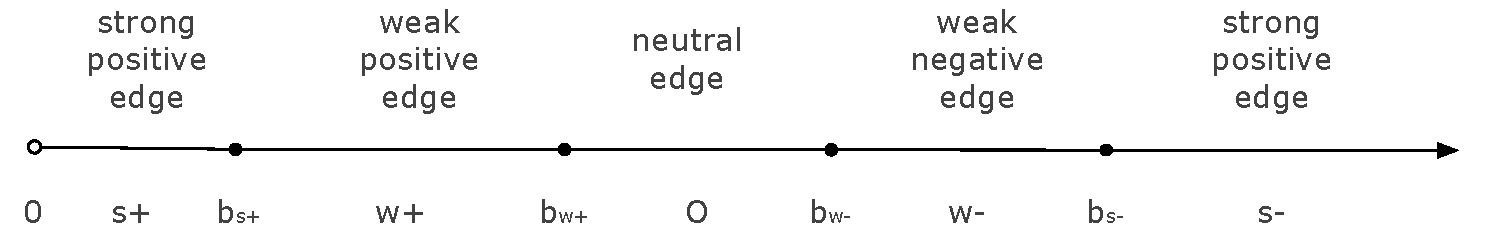
\includegraphics[height=0.7in]{Figs/mapping2.pdf}
\caption{\label{fig:partition}Partitioning of distance domain by boundary
  parameters $\{b_{s+}, b_{w+}, b_{w-}, b_{s-}\}$: distances within $(0,b_{s+}]$ are strong positive; $(b_{s+}, b_{w+})$ weak
  positive, $[b_{w+}, b_{w-}]$ neutral, $(b_{w-}, b_{s-})$
  weak negative, and $ [b_{s-}, \infty)$ strong negative.}

\end{figure}

Similarly, to capture the tolerance rules in Table~\ref{tab:weak_strong_tolerance},
we consider the partitioning of the distance domain given in
Figure~\ref{fig:partition}. We can see that if the following
conditions are satisfied for the boundary parameters: 

\begin{table}[htbp!]
\begin{center}
\caption{\label{tab:constraints}Constraints on the boundary parameters.} 
\begin{tabular}{p{2in}p{2in}}
$b_{w+}  > 2b_{s+}$ & $b_{s-}  > b_{w-} + b_{s+}$  \\
$b_{s-}  > 2b_{w+}$ & $b_{w-}  > b_{w+}+b_{s+}$
\end{tabular}{}
\end{center}
\end{table}
\vspace*{-0.2in}
then the tolerance rules given in
Table~\ref{tab:weak_strong_tolerance} are equivalent to
Definition~\ref{def:gen_tolerance}, and all triads shown in
Table~\ref{tab:imbalanced_extended} are imbalanced according to metric triangle
inequality.

With the concept of relation distance, we are able to express the
structure of a social network by drawing it in the metric
space. The strength of each relation is expressed by the distance
between two of its endpoints. Notice that evesry layout in the metric
space automatically satisfies the metric triangle inequality, and
hence corresponds to a balanced state of the network. We have the following the alternative definition of a balanced network.
\begin{definition}\label{alternative def}
Given a social network $G$, $G$ is balanced if it can be drawn in metric space such that each edge in $G$ has the length of its relation distance.
\end{definition}
%%% Local Variables: 
%%% mode: latex
%%% TeX-master: t
%%% End: 

% Charpter on Convergence Model
% 1. Motivations not restricted to a pure theoretical aspect, as it provides predictive attributes.
%     1.1 List some of the famous predictive phenomenon
% 2. Describe the intuition, and formulate the model in terms of a MDS problem
%      2.1 Proofs/illustrations of phenomenons in 1.1
%%%%%%%%%%%%%%%%%%%%%%%%%%%%%%%%%%%%%%%%%%%%%%%%%%%%%%%%%%%%%%%%%%% 
%                                                                 %
%                            CHAPTER FOUR                          %
%                                                                 %
%%%%%%%%%%%%%%%%%%%%%%%%%%%%%%%%%%%%%%%%%%%%%%%%%%%%%%%%%%%%%%%%%%% 
 



\chapter{CONVERGENCE MODEL} \label{sec:mathmodel}
\section{Convergence Model}
Researchers have long argued that every social network has a tendency
towards balanced states~\cite{Doreian:02}. The balance aspect of ``network evolution" becomes a non-trivial problem when relationships are measured numerically. Given an initially imbalanced network, it is interesting to see what state the network will converge to. We propose a model that characterizes a social network's convergence in this chapter.

It is noted in social psychology literature that people are reluctant
to make changes in relations as they tend to avoid the effort needed to
make such changes. In a balanced triadic relation, participants are
likely to do nothing and keep their pairwise relations as what they
were. In an imbalanced triadic relation, participants are likely to
make the smallest effort possible to regain triadic balance. We define
the concept of relation cost as the effort one needs to take to
accomplish a certain relation change. Our convergence model is
established based on a unified assumption: every social network
converges in a way that requires as little total change in relations
as possible to reach a balanced state.

By definition~\ref{alternative def}, every layout in the Euclidean
space automatically satisfies the metric triangle inequality, and
hence corresponds to a balanced state of the network.  For an
imbalanced social network, it is not possible to draw it using its
initial relation distances.  Hence, our convergence model aims to
produce a layout of the social network with minimum total relation
cost from the original one.

Let $G=(V,E)$ denote an arbitrary social network, and $G^{*}=(V,
E^{*})$ denote a balanced state of $G$. Let $n*n$ matrix $X$ denote
the layout of $G^{*}$, with each row vector $x_{i}$ denoting node
$i$'s location in $m$-dimensional space. For each pair $(i,j)$,
$\psi(i,j)$ denotes its relation distance in $G$, and $d_{i,j}(X)$
denotes distance between $i$ and $j$ in $X$, i.e., its relation
distance in $G^{*}$.  Given an edge $(i,j)\in E$, we consider the
relation cost on $(i,j)$ is given by:
\[c_{i, j}(X)=w_{\psi(i,j)}*(d_{i,j}(X)-\psi{(i,j)})^2\]
where the weight value is a function of the original distance. The
weight function can take into account the difficulty of changing a
relation. For example, it is generally easier to change a neutral
relation than a positive or negative relation that carries with them
initial bias. The study of optimal weights is beyond the scope of this
thesis. However, we consider three main classes of weights:
\[
 w_{\psi(i,j)}= \left\{ 
  \begin{array}{l l}
    w_{+} & \quad \text{if $\psi(i,j)$ is a positive edge}\\
    w_{O} & \quad \text{if $\psi(i,j)$ is a neutral edge}\\
    w_{-} & \quad \text{if $\psi(i,j)$ is a negative edge}\\
  \end{array} \right.
\]

If $w_{O} << w_{+}$ and $w_{O} << w_{-}$, then neutral edges would
have very little influence on the already established
positive/negative relations.

\begin{definition}
Let $G=(V,E)$ be a social network where $E$ is a set of weighted
edges. Its converged network $G^{*}=(V,E^{*})$ is given by layout
matrix $X$ with $d_{i,j}(X)$ as the relation distance between every
pair $(i,j)$, such that the total relation cost $\sigma(X)$ is
minimized,
\[\sigma(X)= \min_{X} \sum_{i<j \leq n}w_{\psi(i,j)}*(d_{i,j}(X)-\psi{(i,j)})^2\].

\end{definition}
The optimization of relation cost is in fact a Metric
Multidimensional Scaling problem (MDS) by assigning nodes a location
in metric space. The total cost function is called stress in MDS, and
is often minimized through an optimization strategy called {\it stress
  majorization} \cite {Gansner:05}. Stress majorization is an iterative
method that guarantees monotonically decreasing stress in each
iteration, and returns a locally minimum solution.  It is recognized
as a principled technique in the field of graph drawing. The
algorithm, however, requires $O(n^3)$ time and $O(n^{2})$ space. Due
to its complexity, stress majorization is applicable on graphs with
limited size. We discuss the algorithmic problem of stress majorization in Chapter 5.

\section{Predictability of Convergence Model}\label{predictability}
A successful convergence model will help justify the balance tendency of social networks, and hence support the balance theory behind it. Moreover, convergence model inherits a predictive power as it models the dynamic nature of social networks. For example, the strong triadic closure states that two people with a common close friend are very likely to friend each other in the future~\cite{Granovetter:1973}. We have argued in Table~\ref{tab:imbalanced_extended} that triad ``$s+, s+, O$" is imbalanced, it is important to verify if such a triad will converge to ``$s+, s+, +$" accordingly in the convergence model. Some frequently seen dynamic phenomenon in social networks are listed below, which we expect a congruent convergence model will be able to explain. The concept of strong and weak ties follows what is described in Table~\ref{ref:rel_types}. Following the discussion in section~\ref{relation distance}, we partition the relation distance by the same constraints in Table~\ref{tab:constraints}. We illustrate and prove these propositions under our convergence model.

 In the demonstration examples shown in Figure~\ref{demo1}, Figure~\ref{demo2} and Figure~\ref{demo3}, the boundary parameters are chosen as the following: $b_{s+}=0.1,\, b_{w+}=0.5,\,  b_{w-}=0.7,\,b_{s-} = 1.1$. The relation distances of strongly positive relation, weakly positive relation, neutral relation, weakly negative relation, strongly negative relation are picked as 0.1, 0.3, 0.6, 0.9, 1.1 respectively. Notice that the parameters is arbitrarily picked for the purpose of demonstration. Other configurations are legitimate as long as the constraints in Table~\ref{tab:constraints} are satisfied. As it is discussed previously, we constrain $w_{0}$ such that $w_{0}<< \min{\{w_{+}, \, w_{-}\}}$. In the demonstration examples, the weights are chosen as: $w_{+}=w_{-}=1,\, w_{0}=0.001$.
 
 In the proofs below, we denote $G$ as the initial network and $\cal G$ as its balanced state after convergence. The initial distance of a neutral relation is denoted as $\delta_{0}$. Clearly, $b_{w+} \leq \delta_{0} \leq b_{w-}$ holds.
 
\begin{proposition}\label{closure}
Strong Triadic Closure Property. Let $(A,B,C)$ be a triad of interest. If both $(A,B)$ and $(B,C)$ are strongly positive relations in a social network, then $(A,C)$ will be a positive relation in the balanced state.
\end{proposition}
Illustrated in (1) of Figure~\ref{demo1}, initially edges $(0,1)$ and $(1,2)$ are given as strongly positive. In its converged layout, node $0$, node $1$ and node $2$ are on the same line with node $1$ in the middle. Hence, $d_{02}$ is twice as much as $d_{01}$ ($d_{12}$). As a result, $(0,2)$ turns to be a weakly positive edge as desired. 

{\bf Proof.} We need to prove that the initially unconnected $(A,C)$ will become a positive edge in $\cal G$. Also, we need to show $(A,B)$ and $(B,C)$ will remain strongly positive in $\cal G$. 

Initially, $\psi{(A,B)} + \psi{(B,C)} < 2b_{s+}<b_{w+}<\delta_{0} =\psi{(A,C)}$. $A$, $B$, $C$ cannot coexist in the space without change some of the distances. To reach a balanced structure, it is either going to stretch $(A,B)$ and $(B,C)$, or to shrink $(A,C)$ in space. But in either way or a combination of both, the least modification, which indicates the smallest relation cost, occurs when $A$, $B$, $C$ stays in a line with $B$ in the middle. 
Let the length of both $(A,B)$ and $(B,C)$ be $l_{1+}$ and $l_{2+}$, and the length of $(A,C)$ be $l_{0}$. The total relation cost should be the following.
\[
\sigma(l_{1+}, l_{2+} l_{0}) = \min_{l_{1+},l_{2+}, l_{0}} w_{0}(l_{0}-\delta_{0})^2 + w_{+}(l_{1+}-\psi{(A,B)})^2+ w_{+}(l_{2+}-\psi{(A,B)})^2
\]
\[
\text{subject to  } l_{0}=l_{1+}+l_{2+}.
\]
The optimization problem can be rewritten as the following,
\[
\sigma(X)= \min_{X}\, 1/2X^{\top}HX+C^{\top}X+ \alpha,
\]
where $\alpha$ is a constant and
\[
 X =
 \begin{pmatrix}
  l_{1+}  \\
  l_{2+},
 \end{pmatrix},
  H =
 \begin{pmatrix}
  2(w_{0}+w_{+}) & 2w_{0}\\
  2w_{0} & 2(w_{0}+w_{+})
 \end{pmatrix},
  C =
 \begin{pmatrix}
  -2(w_{0}\delta_{0}+w_{+}\psi(A,B))  \\
  -2(w_{0}\delta_{0}+w_{+}\psi(A,C))
 \end{pmatrix}.
\]
Let  $\frac{\mathrm d}{\mathrm d X} \big( \sigma(X) \big)=0$. We have $X=-H^{-1}C$,
\[
  X=\left\{ 
  \begin{array}{l l}
    {l_{1+}} = {{w_{0}\delta_{0}+(w_{0}+w_{+})\psi(A,B)-w_{0}\psi(B,C)} \over {2w_{0}+w_{+}}}\\
    {l_{2+}}={{w_{0}\delta_{0}+(w_{0}+w_{+})\psi(B,C)-w_{0}\psi(A,B)} \over {2w_{0}+w_{+}}}
  \end{array} \right.\text{ ,}
\]
and
\[
l_{0}=l_{1+}+l_{2+} ={{2w_{0}\delta_{0}+w_{+}(\psi(A,B)+\psi(B,C))} \over {2w_{0}+w_{+}}} \text{ .}
\]
By constraint $w_{0}<<w_{+}$, we have
\[
{l_{1+}}=\psi(A,B)+{{w_{0}(\delta_{0}-\psi(A,B)-\psi(B,C))} \over {2w_{0}+w_{+}}} \simeq \psi(A,B)
\]
Similarly, ${l_{2+}} \simeq \psi(B,C)$. Hence, both $(A,B)$ and $(B,C)$ will remain strongly positive. Now, $l_{0} \simeq \psi(A,B)+ \psi(B,C) < b_{w+}$, and therefore $(A,C)$ will become a positive relationship. $\Box$\\

\begin{figure}[th]
\centering
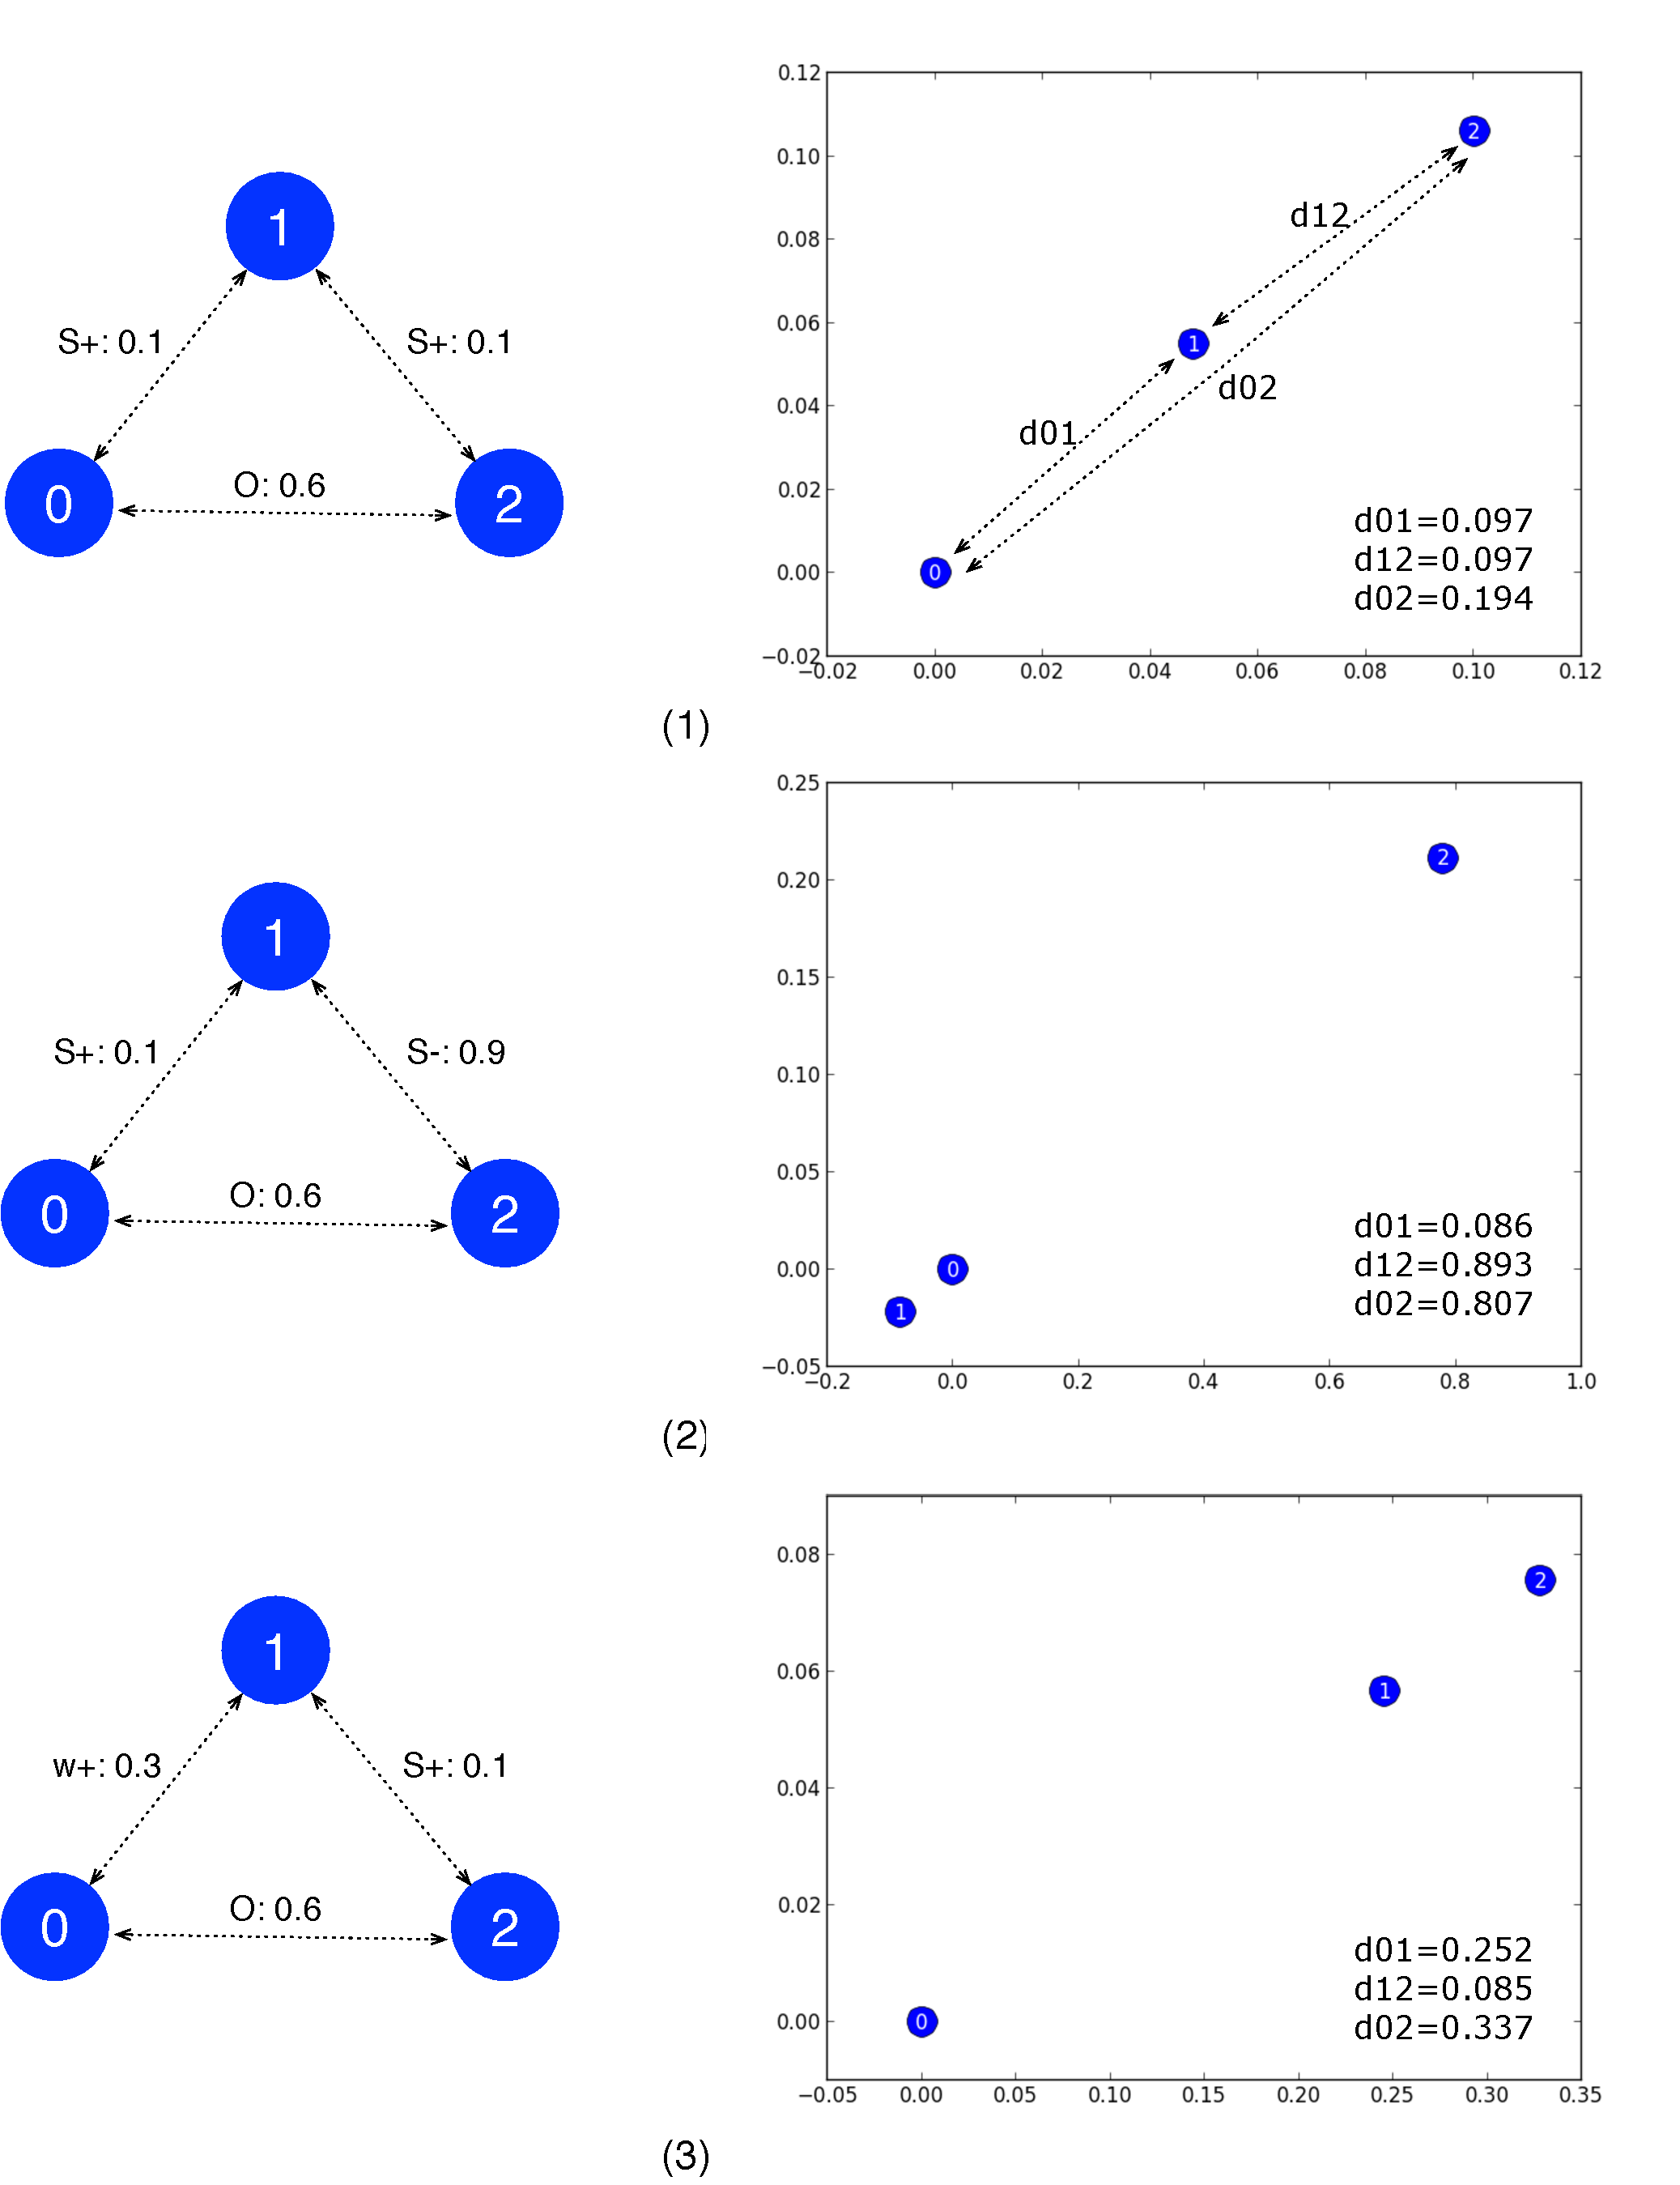
\includegraphics[height=5.5in]{Figs/demo1.pdf}
\caption{\label{demo1}The demonstration experiments of Propositions~\ref{closure}, \ref{neutralization} and \ref{attenuation}. Each blue ball has a white number $i$ in it, indicating node $i$. The initial state of each triad is shown in figures on the left, and the corresponding converged layouts on the right.}
\end{figure}
\begin{proposition}\label{neutralization}
Neutralization Property. Let $(A,B,C)$ be a triad of interest. If $(A,B)$ is strongly positive and $(B,C)$ is strongly negative, then $(A,C)$ will be negative in the balanced network, and the strength of $(A,C)$ should be no stronger than the strength of $(B,C)$.   
\end{proposition}
The first part of the neutralization property can be seen as a twin property of strong triadic closure with negative sign. It says if A has a friend B and a strong enemy C, then B and C will not get along in the long run. The second part is an inference assumption; one argument for the assumption is: ``the later established disliking is not likely to be stronger than the original hatred that causes the disliking". 

Illustrated in (2) of Figure~\ref{demo1}, initially edge $(0,1)$ is given as strongly positive while edge $(1,2)$ is given as strongly negative. In its balanced layout, node $0$, node $1$ and node $2$ are on the same line with node $0$ in the middle. Hence, $d_{02}$ equals $d_{12}-d_{01}$, which is in the range of negative relations. 

{\bf Proof.} We need to prove $(A,C)$ will become a negative edge in $\cal G$, and that $(A,C)$ will not be longer than $(B,C)$ in metric space. Also, we need to prove $(A,B)$ and $(B,C)$ will remain what they were in $\cal G$. 

By similar arguments in the proof of Proposition~\ref{closure}, $A$, $B$, $C$ cannot coexist in the space without change some of the distances. To reach a balanced structure, it is either going to stretch $(A,B)$ and $(A,C)$, or to shrink $(B,C)$ in space. But in either way or a combination of both, the least modification, which indicates the smallest total relation cost, occurs when $A$, $B$, $C$ stays in a line with $A$ in the middle. Let the length of $(A,B)$ be $l_{+}$, the length of $(B,C)$ be $l_{-}$ and the length of $(A,C)$ be $l_{0}$. The total relation cost on ($A$, $B$, $C$) during the convergence should be the following.
\[
\sigma(l_{+}, l_{0}, l_{-}) = \min_{l_{+}, l_{0}, l_{-}} w_{0}(l_{0}-\delta_{0})^2 + w_{+}(l_{+}-\psi(A,B))^2+w_{-}(l_{-}-\psi(B,C))^2
\]
\[
subject\,\,to  \quad l_{0}+l_{+}=l_{-}.
\]
The optimization problem can be rewritten as the following,
\[
\sigma(X)= \min_{X}\, 1/2X^{\top}HX+C^{\top}X+ \alpha,
\]
where $\alpha$ is a constant and
\[
 X =
 \begin{pmatrix}
  l_{0}  \\
  l_{+},
 \end{pmatrix},
  H =
 \begin{pmatrix}
  2(w_{0}+w_{-}) & 2w_{-}\\
  2w_{-} & w(w_{+}+w_{-})
 \end{pmatrix},
  C =
 \begin{pmatrix}
  -2(w_{0}\delta_{0}+\psi(A,C))  \\
  -2(w_{+}\psi(A,B)+\psi(B,C))
 \end{pmatrix}\text{ .}
\]
Let  $\frac{\mathrm d}{\mathrm d X} \big( \sigma(X) \big)=0$. We have $X=-H^{-1}C$, 
\[
  X=\left\{ 
  \begin{array}{l l}
    {l_{0}} = {{(w_{+}w_{0}+w_{0}w_{-})\delta_{0}+w_{+}\psi(A,C)-w_{+}w_{-}\psi(A,B)} \over {w_{0}w_{+}+w_{+}w_{-}+w_{0}w_{-}}}\\
    {l_{+}}={{(w_{+}w_{0}+w_{+}w_{-})\psi(A,B)+w_{0}\psi(A,C)-w_{0}w_{-}\delta_{0}} \over {w_{0}w_{+}+w_{+}w_{-}+w_{0}w_{-}}}
  \end{array} \right. \text{ ,}
\]
and
\[
{l_{-}}={{w_{+}w_{0}\psi(A,B)+w_{+}w_{0}\delta_{0}+(w_{+}+w_{0})\psi(A,C)} \over {w_{0}w_{+}+w_{+}w_{-}+w_{0}w_{-}}}\text{ .}
\]
By constraints $w_{0}<<\min{\{w_{+},w_{-}\}}$  and $w_{-}=1$, we have
\[
{l_{0}} \simeq {{w_{+}\psi(A,C) - w_{+}w_{-}\psi(A,B)} \over {w_{+}w_{-}}} = {\psi(A,C) \over {w_{-}}} - \psi(A,B)=\psi(A,C)-\psi(A,B)\text{ ,}
\]
\[
{l_{+}} \simeq \psi(A,B) \text{ ,}
\]
\[
{l_{-}} \simeq {\psi(A,C) \over {w_{-}}}=\psi(A,C) \text{ .}
\]
Hence, $(A, B)$ will remain strongly positive, $(B,C)$ will remain strongly negative and $(A,C)$ will be no longer than $(B,C)$. Since $\l_{0} \simeq \psi(A,C) - \psi(A,B) >b_{s-}-b_{s+}>b_{w-}$, $(B,C)$ will be a negative relation after convergence. $\Box$\\


\begin{proposition}\label{attenuation}
Attenuation Property. Let $(A,B,C)$ be a triad of interest. If $(A,B)$ and $(B,C)$ are both positive, then $(A,C)$ will be non-negative in balanced network, and the strength of $(A,C)$ should be no stronger than the strength of either $(A,B)$ or $(B,C)$.
\end{proposition}
The first part of the propagation attenuation property can be seen as a weaker triadic closure property. It says that if two people have a common friend, then based on this information alone, they cannot be enemies. The second part, a similar inference assumption as the one in Proposition~\ref{neutralization}, can be explained by ``the later established liking is not likely to be stronger than the original brotherhood that invokes the liking". 

Illustrated in (3) of Figure~\ref{demo1}, initially edge $(0,1)$ is weakly positive while edge $(1,2)$ is strongly positive. Similar to the situation in (1), $d_{02}=d_{01}+d_{12}$, which is in the range of weakly positive relations. Also, of course, $d_{02}>\max {\{d_{01}, d_{12}\}}$, which agrees with the attenuation property.

{\bf Proof.} Let $(A,B)$ , $(B,C)$ be positive edges. Suppose that $\psi(A,B)$ , $\psi(B,C)$, $\psi(A,C)$ still violate the triangle inequality. By the same arguments in the proof of Proposition~\ref{closure}, we still conclude that in the balanced network $(A,C)$ will be a positive edge, with its strength no stronger than the strength of either $(A,B)$ or $(B,C)$. Otherwise, since $(A,B)$ , $(B,C)$, $(A,C)$ are able to coexist with its original relation distance, all of the three edges will remain what they were in the balanced network with a total relation cost of $0$. Hence, $(A,C)$ will remain as a neutral edge. $\Box$\\
\begin{figure}[th]
\centering
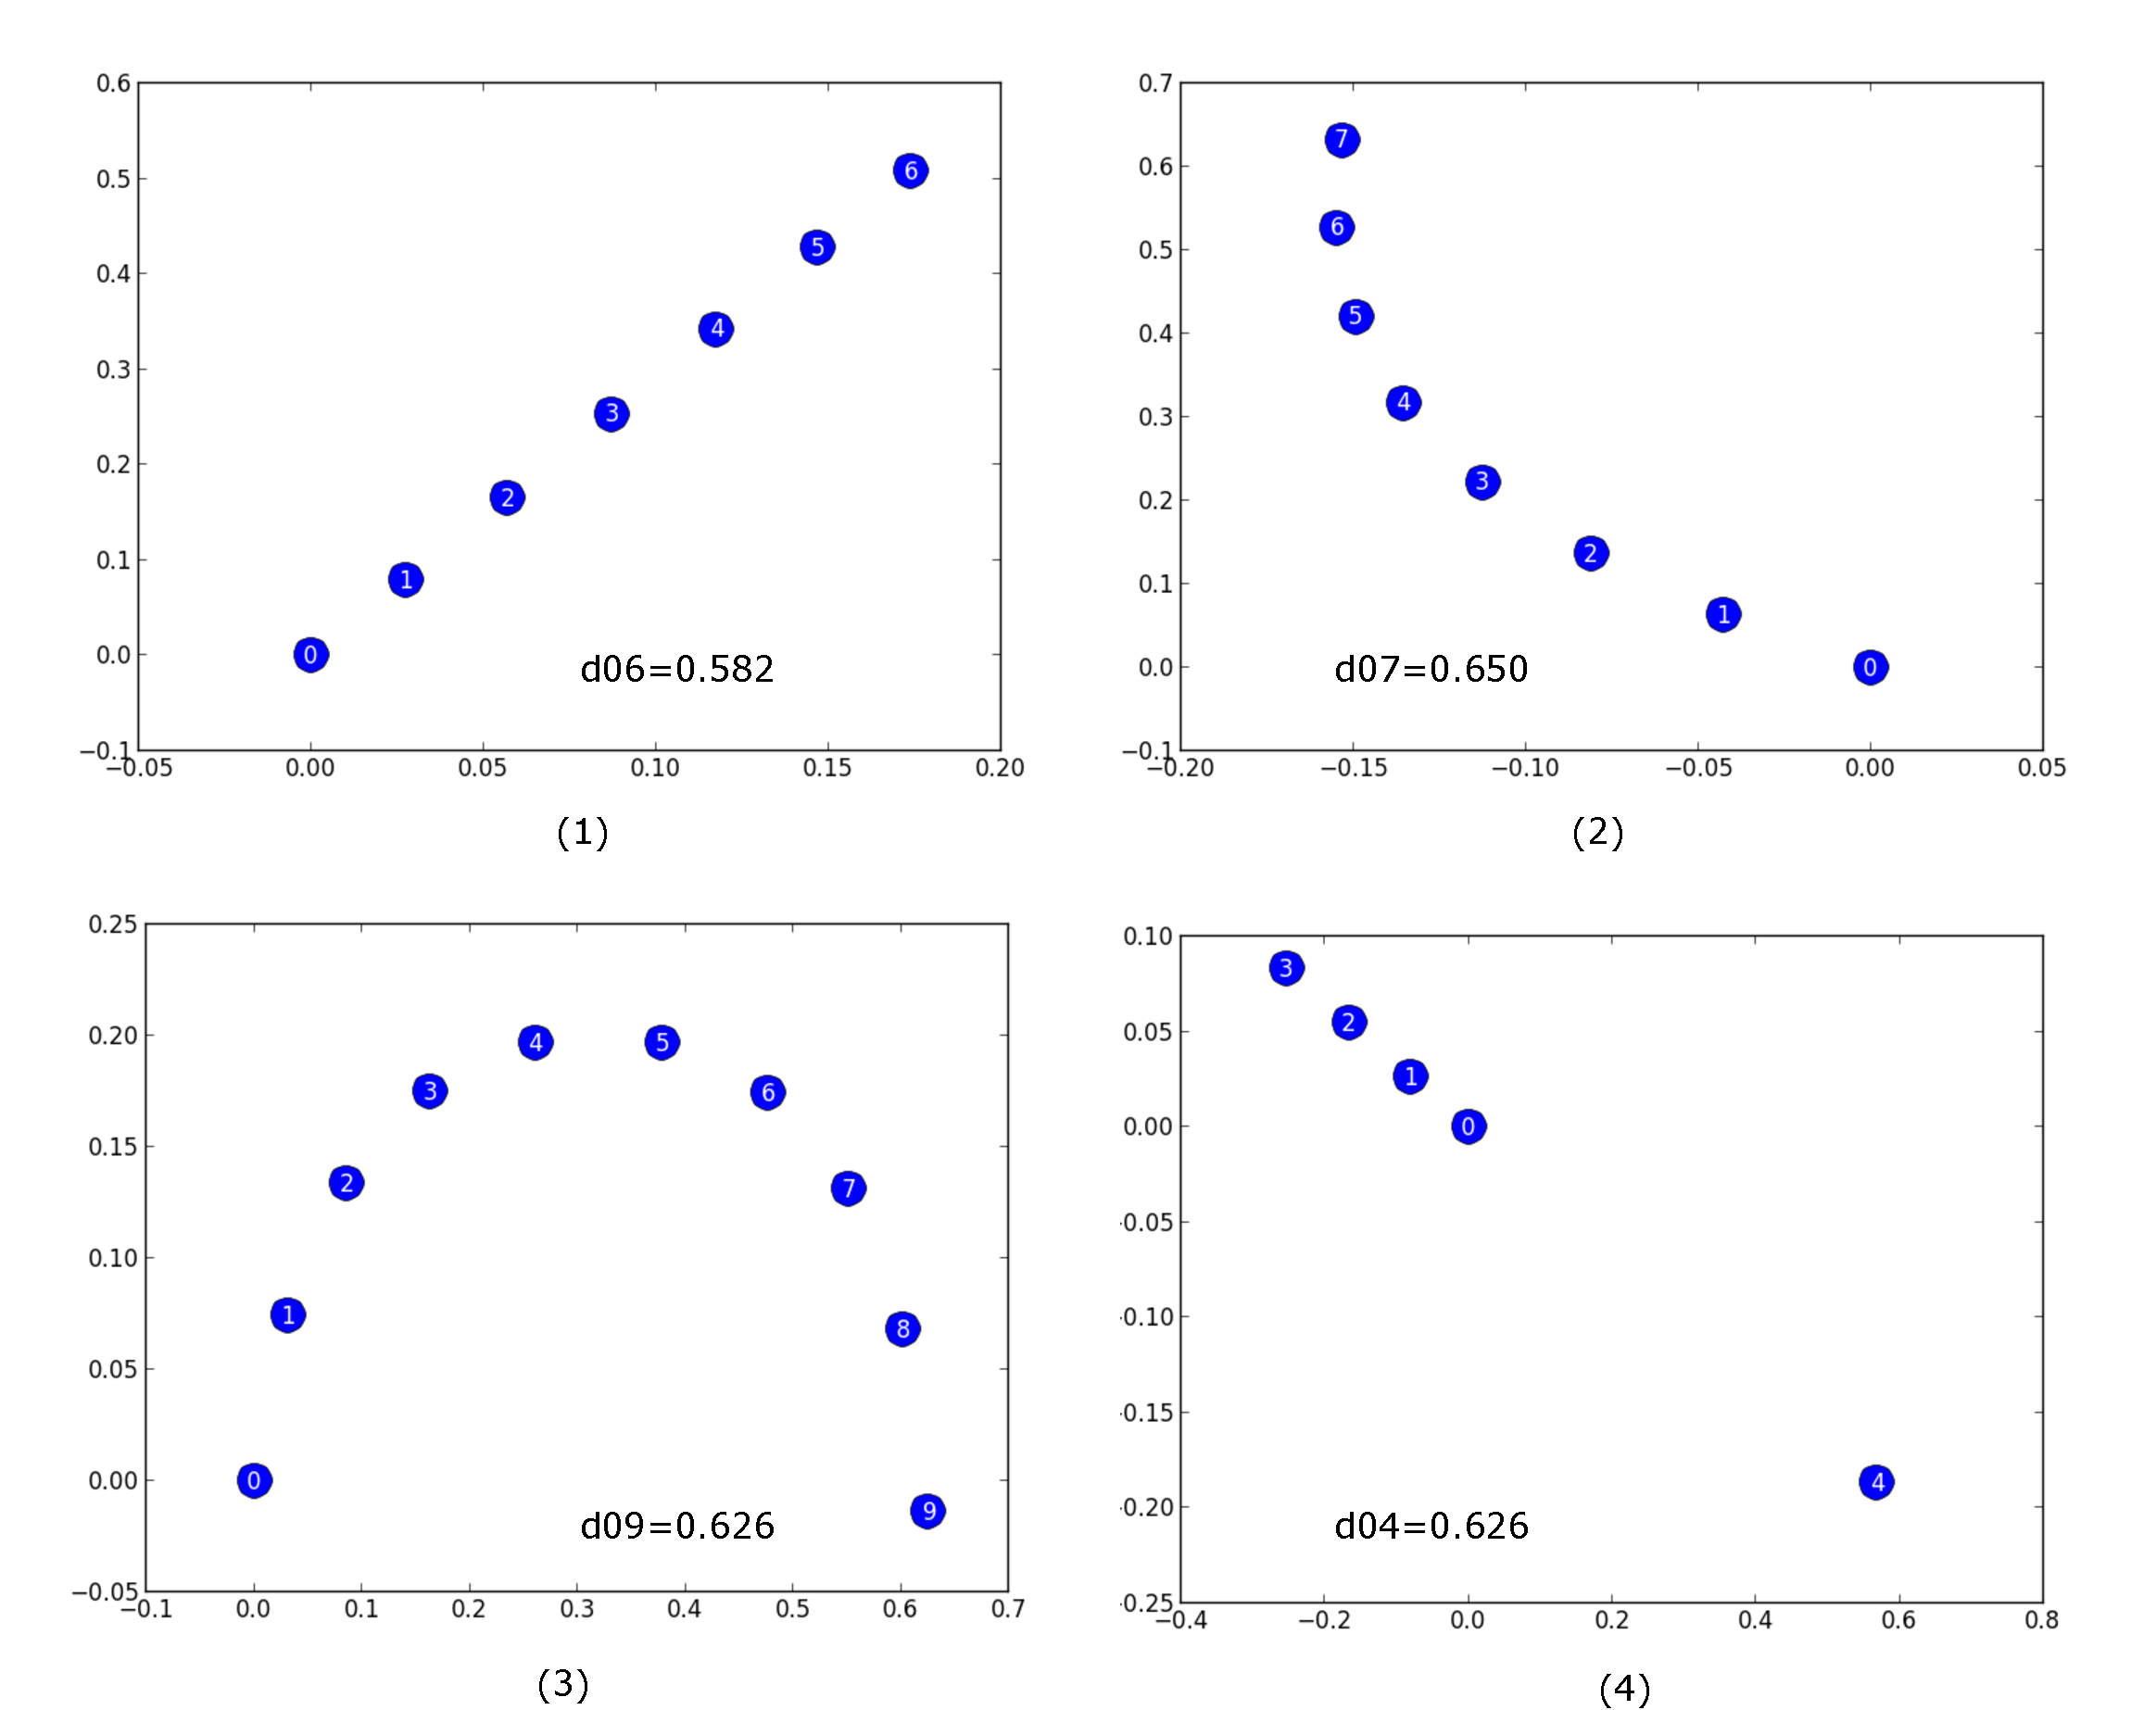
\includegraphics[height=5.0in]{Figs/demo2.pdf}
\caption{\label{demo2}The demonstration experiments of Corollary~\ref{positive path} and \ref{negative path}. Each blue ball has a white number $i$ in it, indicating node $i$'s location in its converged layout.}
\end{figure}
By Proposition~\ref{neutralization}  and Proposition~\ref{attenuation},  we further have the following two corollaries regarding positive and negative paths.
\begin{corollary}\label{positive path}
Positive Path. Given a path that consists of positive edges only, the positive relation will propagate with its strength being attenuated along the path, until it becomes a neutral relation.
\end{corollary}
Let $A_{1},A_{2},...,A_{n}$ be a positive path, such that every $(A_{1}, A_{2})$ is a positive relation. The corollary states that every $(A_{1}, A_{k})$ will be a non-negative relation, and that $(A_{1}, A_{k-1})$ will be positively stronger than $(A_{1}, A_{k})$.
\begin{corollary}\label{negative path}
Negative Path. Given a path that consists of only one negative edge, the relation between the end nodes of the negative path is non-positive in the balanced network. 
\end{corollary}
We demonstrate the transitivity and attenuation along a Positive Path in (1) (2) (3) of Figure~\ref{demo2}. (1) of Figure~\ref{demo2} shows the converged layout of a positive path consisting of $6$ strongly positive relations. In this configuration, since the sum of all $6$ distances is smaller than the relation distance of a neutral edge, all nodes stay on the same line. Clearly, $d_{06} > d_{05}>...>d_{02}$, which agrees with the attenuation property. $d_{06}$ turns to be in the range of neutral relations, which indicating the relationship between node $0$ and node $6$ becomes neutral.  

(2) (3) of Figure~\ref{demo2} show the converged layout of a positive path consisting of $7$ and $9$ strongly positive relations respectively. In such cases,  the sum of all $7$ or $9$ distances becomes larger than the relation distance of a neutral edge. As a result, the layout of nodes curves. Both $d_{07}$ and $d_{09}$ are in the range of neutral relations. Moreover, $d_{07}$ is consistently larger than $d_{09}$ in our experiments, indicating the distance between two endpoints of the positive path is non-increasing w.r.t. the path length. The empirical results of (2)(3) show the non-negativeness of the relationship between the endpoints of a positive path.

(4) of Figure~\ref{demo2} is the converged layout of a negative path, in which $(3,4)$ is the only negative edge. Similar to positive path, it has a non-positive relationship between its two endpoints.
\begin{figure}[th]
\centering
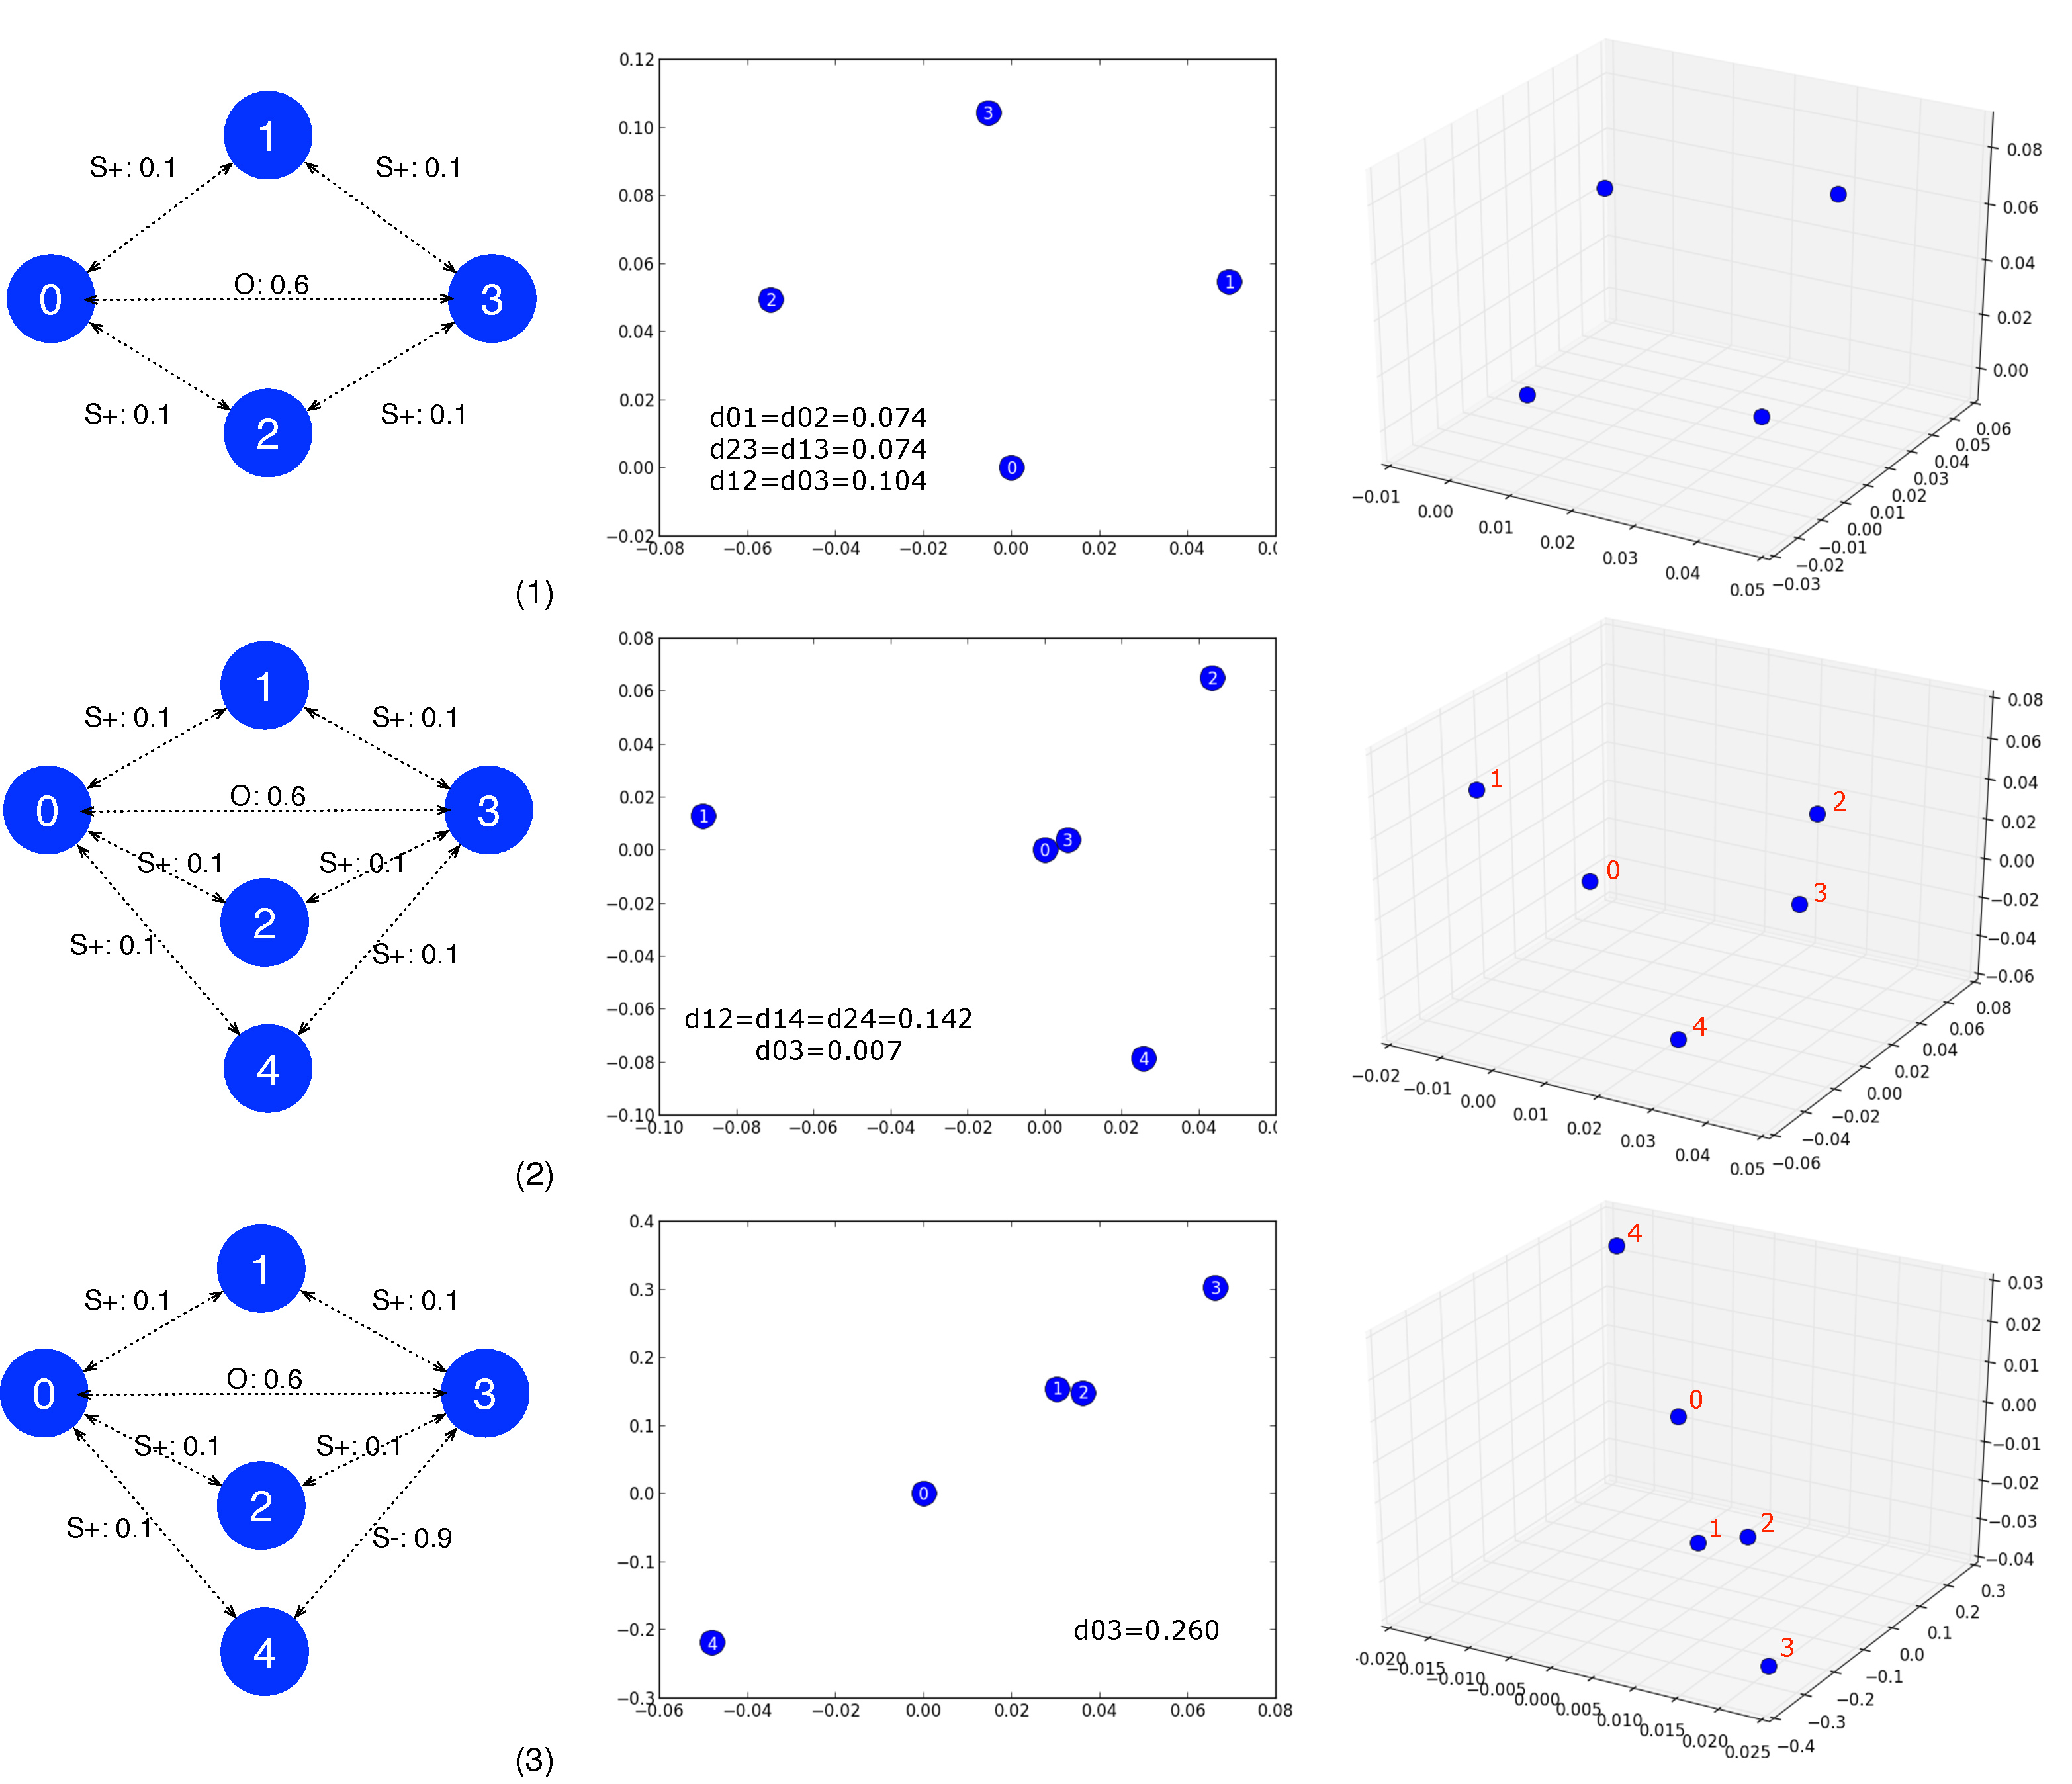
\includegraphics[height=5.0in]{Figs/demo3.pdf}
\caption{\label{demo3}The demonstration experiments of Proposition of Aggregation. Each blue ball has a white number $i$ in it, indicating node $i$. The initial state of each triad is shown in figures on the left, the corresponding converged layouts in 2-D space is shown in the middle, and the corresponding converged layouts in 3-D space is shown on the right.}
\end{figure}
\begin{proposition}\label{aggregation}
Aggregation Property. Suppose there are multiple positive and negative paths between two nodes, then adding one more positive path between them will make their relation more positive while adding one more negative path will make the relation more negative.
\end{proposition}
Aggregation property is a generalization of ``people with more common friends are more likely to become friends". It says if two people A,B have more (direct or indirect) friends in common, then they are more likely to be friends, or less likely to be enemies. On the other hand, if they have more conflicting people in common, who are (direct or indirect) friends of A and (direct or indirect) enemies of B, then they are more likely to be enemies, or less likely to be friends.  

To illustrate the Property of Aggregation, we run $3$ different tests. In the first experiment shown in (1) of Figure~\ref{demo3}, edges $(0,1),\,(0,2),\,(1,3),\,(2,3)$ are given as strongly positive initially.  The converged layout forms a square, and $d_{03}=\sqrt{2}{d_{01}}$. Obviously, $d_{03}$ is in the range of positive relations. Moreover, $d_{03}$ is smaller than $d_{02}$ in (1) of Figure~\ref{demo1}, which indicates adding a common friend between two people will grant a better chance to them to become friends. In the second experiment shown in (2) of Figure~\ref{demo3}, we add another positive path ${0,4,2}$. The converged layout is still symmetric, but the distance between node $0$ and node $3$ becomes very close, which agrees with the concept of aggregation. In the third experiment shown in (3) of Figure~\ref{demo3}, we add a negative path instead. In the converged layout, the distance between node $0$ and node $3$ becomes larger than $d_{02}$ in (1) of Figure~\ref{demo1}, which indicating adding a conflicted common neighbor between two people will deteriorate their relationship.

When the number of nodes is more than $3$, a two-dimensional drawing is not necessarily able to express the layout of minimum relation cost. For example, in (2) of Figure~\ref{demo3}, $d_{03}$ would be larger if drawing in a 3-D space. Due to the limit of dimensionality, node $0$ and node $3$ are forced to squeeze together. In studying the effects of dimensionality, we repeat the same aggregation demonstrations in 3-D space. In (1) of Figure~\ref{demo3}, the layout still forms a square. In (2) of Figure~\ref{demo3}, the layout forms a  triangular bipyramid, and the distance between node $0$ and node $3$ becomes reasonably small, but is still smaller than it is in (1) of Figure~\ref{demo3}. In (3) of Figure~\ref{demo3}, the distance between node $0$ and node $3$ is slightly larger than it is in (1) of Figure~\ref{demo3}, showing a more reasonably deterioration of relationship by adding a negative path.

{\bf Proof. } We present the general idea of the proof. See appendix for the full proof. 
Initially, strongly positive relations $(A, B)$, $(B, D)$ are given. By Proposition~\ref{closure}, the length of $(A,D)$ will be approximately $\psi(A,B)+\psi(B,D)$ in the balanced network.

Suppose one more positive paths is added between $A$ and $D$. For example, strong positive edges $(A,C)$ and $(C,D)$ are added. Neutral edge $(B,C)$ needs to stretch out to reach their initial length $b_{w+}$. But if edge $(B,C)$ stretches more, edge $(A,D)$ has to stretch less in space. In the balanced network $\cal G$, $A,B,C,D$ will form a quadrilateral in the Euclidean space. Hence, the length of $(A,D)$ will be smaller than $\psi(A,B)+\psi(B,D)$.

Moreover, with more neutral edges like $(B,C)$ on the multi-plane that is vertical to $(A,D)$, the network structure will be balanced at a point where $(A,D)$ is less stretched, so that the total relation cost is minimized. 

On the other hand, if adding one more negative path between $A$ and $D$, then equivalently a non-positive relation will be added between them according to corollary~\ref{negative path}. If it is a negative relation, $(A,D)$ will be directly stretched out, because negative relation is longer than neutral relation in metric space. $\Box$
%Charpter on algorithms of stress majorization
%     Reivew of SM
% 1. SM in terms of sparse matrix
% 2. An approximation algorithms
%%%%%%%%%%%%%%%%%%%%%%%%%%%%%%%%%%%%%%%%%%%%%%%%%%%%%%%%%%%%%%%%%%% 
%                                                                 %
%                            CHAPTER FIVE                          %
%                                                                 %
%%%%%%%%%%%%%%%%%%%%%%%%%%%%%%%%%%%%%%%%%%%%%%%%%%%%%%%%%%%%%%%%%%% 
 



\chapter{ALGORITHMS FOR STRESS MAJORIZATION} \label{sec:mathmodel}
In this chapter, we review the problem of stress majorization in the MDS literature~\cite{Gansner:05}. Stress majorization is recognized as a principled technique in graph drawing~\cite{Leeuw:77}. Due to its complexity, however, classic stress majorization is applicable on graphs with limited size. Modern social networks usually consist of over $10^5$ nodes, which are typically infeasible for stress majorization. We discuss two algorithms that together give solution to our convergence model in the context of large social networks. 

\section{Review of stress majorization}
Following Gansner's description, we denote the d-dimensional location matrix as $X$~\cite{Gansner:05}. Let node $i$'s location be $X_{i}$. The MDS problem is to minimize the following stress function
\begin{equation}\label{stress}
stress(X)=\sum_{i<j} w_{ij} (||X_{i}-X_{j}|| - d_{ij})^{2}\,,
\end{equation}
where $w_{ij}$ are weights and $d_{ij}$ denote the ideal distance between $i$ and $j$. 
There are many ways to minimize $stress(X)$. Among them, De Leeuw's stress majorization technique is considered to be a major achievement on the subject. The iterative majorization method at each step minimizes a simple convex function, which guarantees a monotonically convergent solution~\cite{Leeuw:77}. 
In application, the majorization process involves solving the following equation iteratively. For a detailed analysis of Stress Majorization, please refer to Appendix A. 

\begin{equation}\label{recursive}
L^{w}X(t+1)=L^{X(t)}X(t),
\end{equation}
where $L^{w}$ and $L^{X(t)}$ are given by
\[
 L_{i,j}^{w}=\left\{ 
  \begin{array}{l l}
    -w_{ij} \quad & i \neq j\\
    \sum_{k \neq i}w_{ik} \quad &i=j 
  \end{array} \right. \text{,}\quad
  L_{i,j}^{X(t)}=\left\{ 
  \begin{array}{l l}
    -w_{ij}d_{ij}/||X(t)_{i}-X(t)_{j}|| \quad & i \neq j\\
    -\sum_{j \neq i}L_{i,j}^{X(t)} \quad &i=j 
  \end{array} \right. \text{ .}\]

At each iteration, $L^{w}$ is constant throughout the process, whereas matrix $L^{X(t)}$ needs to be computed recursively.
While stress majorization is an effective and accurate optimization strategy, it is not feasible in very large networks. Solving Equation~\ref{recursive} in each iteration requires the computation of a fully dense matrix, which in total requires $O(n^3)$ time and $O(n^{2})$ space. For network of node number $> 10^{5}$, direct implementation of stress majorization becomes impossible.
\section{Stress Majorization in Large Social Networks}
We discuss two algorithms to solve the optimization given in Equation~\ref{stress} in large social networks. 

{\bf Algorithm 1.} First, we note that social networks are usually sparse. In other words, there are a lot more ``no-links" than ``real links". If we set these neutral edge's weight $w_{O}$ to $0$, $L^{w}$ will be a sparse matrix. Moreover, the right side of the iteration, $L^{X(t)}X(t)$, can be expanded to the following:
\begin{equation}\label{rightside}
(L^{X(t)}X(t))_{i}= \sum_{j \neq i} w_{ij}d_{ij} \frac {X_{i}-X_{j}}{||X_{i}-X_{j}||} .
\end{equation}
Hence, we will only need to sum up the terms corresponding to ``real links" to get $L^{X(t)}X(t)$. Let the average degree of a social network be $k$, computing $L^{X(t)}X(t)$ only requires $O(kn)$. The cost to solve the linear equation~\ref{recursive} with sparse matrix $L^{w}$ is usually much less than $(2/3n^{3})$, depending on the patterns of $L^{w}$. As a result, the problem is likely to become feasible in large social networks.

However, we cannot simply we set $w_{O}$ to $0$, because otherwise relationship changes regarding initially neutral relations would add zero relation cost. As a result, arbitrary changes over initially neutral relations would occur, and properties such as transitivity of positive relationships would not necessarily hold anymore. 

Our second observation is inspired by the famous small world phenomena~\cite{Kleinberg:00},\cite{Watts:98}. If two people are somehow connected by a path of relations, the path is often of very short length. In the setting of online social networks, we regard two people who are connected by paths of more than length 4 distant from each other, and hence assume their relationship will remain neutral over the convergence. As a result, we only need to consider neighbors of each node within two links, which is in average $k^2$ in number. Under this constraint, computing $L^{X(t)}X(t)$ requires $O(k^{2}n)$ while $L^{w}$ is still sparse ($k^{2}$n non-zero entries). The convergence problem is solvable in large social networks while the principle of relation cost minimization is not violated. 
\begin{algorithm}\label{alg1}
\KwData{$G, w_{+}, w_{-}, w_{O}, \theta$}
\KwResult{$X$ }
Create a sparse matrix $L^{w}$\;
\For{each node $i$ in $G$}{
\For{each direct neighbor $j$ of node $i$}{
\eIf{$(i,j)$ is a positive edge}{
set $L^{w}_{ij}=w_{+}$\;
}{
set $L^{w}_{ij}=w_{-}$\;
}
}
\For{each 2-step neighbor $k$ of node $i$}{
set $L^{w}_{ij}=w_{O}$\;
}
}
 Initialize $X^{'}$ as a random layout\;
\Repeat{$(stress(X)-stress(X^{'}))/stress(X) < \theta$}{
$X=X^{'}$\;
compute $stress(X)$ by Equation~\ref{stress}\;
compute $X^{'} = (L^{w})^{-1} L^{X}X$ following Equation~\ref{recursive} and Equation~\ref{rightside}\;
compute  $stress(X^{'})$ by Equation~\ref{stress}\;
}
\Return X\;
 \caption{Stress Majorization with sparse $L^{w}$}
\end{algorithm}
 {\bf Algorithm 2.} The second algorithm is inspired by Khoury's latest work. They first proposed the problem of drawing very large graphs by low-rank stress majorization \cite{Khoury:12}. Our algorithm is a refined version of their work, designed for applications in large social networks. In the setting of a social network, $X$ denotes the location matrix of the each node, and $w_{ij}$ and $d_{ij}$ are attributes regarding social links. Many social networks, such as the ones with signed edges (positive/negative), have limited type of edges. Hence, we assume that both $w_{ij}$ and $d_{ij}$ have finite values. Precisely, each $w_{ij}d_{ij}$ has finite values. For example, in a social network with signed edges, $w_{ij}$ and $d_{ij}$ should have only two values corresponding to a positive edge and a negative edge. In graph drawing, $w_{ij}d_{ij}=1$ is typically assumed \cite{Gansner:05}, \cite{Khoury:12} . We do not have such an assumption here. 

The high complexity of stress majorization comes from computing Equation~\ref{recursive} iteratively. The computation can be divided into two parts. 1. Solve equation $L^{w}X(t+1)=b$, assuming $b=L^{X(t)}X(t)$ is given; 2. Compute $L^{X(t)}X(t)$ efficiently. 

For the first sub-problem, Khoury first proposed a low-rank SVD based approximation approach. Inspired by the work by Drineas, they used a random sampling technique to approximate $L^{w}$ with only a small fraction of its columns \cite{Drineas:04}. Every matrix $M$ admits a SVD decomposition of the form $M=U \Sigma V^{T}$, where $U$ and $T$ are orthogonal matrixs. When the diagonal elements of $\Sigma$ are in non-increasing order, setting all but the first $k$ values of $\Sigma$ to zero yields a sequence of increasingly better approximation of $M$ as $k$ increases. If most values of $\Sigma$ are relatively close to zero, zeroing them does not change $M$ much. For matrix $L^{w}$, it satisfies equation $L^{w}=D^{w}+O^{w}$, where $O^{w}$ is an off-diagonal matrix with each element $O^{w}_{ij}=-wij$ and $D^{w}=- diag(O^{w} {\bf 1})$ is a diagonal matrix. Since matrix $D^{w}$ depends on $O^{w}$ and $O^{w}$ has better $k-rank$ approximation than original $L^{w}$, we approximate $O^{w}$ instead. Consequently, $L^{w}$ is represented by the following form
\begin{equation}
L^{w}=D^{w}+O^{w}=-diag(U\Sigma V^{T} {\bf 1}) + U\Sigma V^{T}.
\end{equation} 
Our next step is to approximate $O^{w}$ by the k most significant values of $\Sigma$. In other words, we will only need to store two $n \times k$ matricies and a $k \times k$ matrix. 

Since $L^{w}$ is singular, $L^{w}X(t+1)=b$ is undetermined. We consider its minimum norm solution, $L^{w+}b$, where $L^{w+}$ is the Moore-Penrose Pseudo-inverse of $L^{w}$ \cite{Golub:96}. Since matrix $L^{w}$ is singular and that its null space is based by exactly ${\bf 1}$, we project $L^{w}$ out to circumvent the singularity.
\begin{equation}
L^{w+}=(L^{w} + {\bf {1}{1}^{T}})^{-1} - {\bf {1}{1}^{T}}
\end{equation}
\begin{equation}
(L^{w} + {\bf {1}{1}^{T}})^{-1} = (U \Sigma V^{T} + D^{w} + {\bf {1}{1}^{T}})^{-1}
\end{equation}
Let $A=D^{w}+{\bf {1}{1}^{T}}$, and by the Woodbury Matrix Identity \cite{Hager:89},
\begin{equation}
(L^{w} + {\bf {1}{1}^{T}})^{-1} =(A+ U \Sigma V^{T})^{-1} = A^{-1} -A^{-1} U T_{1}^{-1} V^{T} A^{-1},
\end{equation}
where 
\[
A^{-1}=(D^{w})^{-1} - T_{2}T_{3}^{-1}T_{2}^{T},
\]
\[
T_{1}=(\Sigma^{-1} + V^{T}A^{-1}U),
\]
\[
T_{2}=(D^{w})^{-1}{\bf {1}},
\]
\[
T_{3}=1+ \langle {\bf {1}}, T_{2} \rangle .
\]
Since $D^{w}$ can be written as $diag(U \Sigma V^{T} {\bf 1})$, the above computation only involves matrix $\Sigma$, $U$ and $V$. If only the k most significant values of $\Sigma$ is taken, $L^{w+}b$ can be efficiently computed. Specifically, the computational cost is $O(k^{3})$. The next question is how to accurately approximate the SVD of  $O^{w}$. 

In~\cite{Drineas:04}, the authors propose a randomized algorithm to approximate the SVD of a matrix by only sampling $k$ columns of the matrix. In particular,  each column $M_{i}$ of a matrix $M$ is sampled with a probability of $p_{i}=||A_{i}||^{2}/||A||^{2}_{F}$. Each picked column is then scaled by a factor of $1/ \sqrt{k p_{i}}$, the obtained $n \times k$ matrix $\hat {M}$ is shown to approximate $M$ with good error bound. The computation of SVD of  such $\hat {M}$ requires $O(nk^{2})$ time.

Given the assumption that $w_{ij}$ has limited number of values, we are able to compute the 2-norms without accessing every item of $L^{w}$. For example, in the social network with signed edges, for each node (column) $i$, its norm can be computed by counting the number of positive edges and negative edges it connects to, which takes $O(dn)$ where $d$ is the average degree. In many applications, we expect the average degree is much smaller than $n$. 

In total, we can see the total running time of the first part algorithm is $O(k^{3}+nk^{2}+nd)$, where $k$ is a selected rank and $d$ is the average degree of the network.

For the second sub-problem, the computation of $L^{X(t)}X(t)$ can be well approximated using Barnes-Hut algorithm of n-body problem with high efficiency~\cite{Barnes:86}. As it is in Equation~\ref{rightside}, $L^{X(t)}X(t)$ is a weighted sum of unit vector to $i$ from every other nodes. This can be treated as an n-body problem, where every weighted vector is the force every node $j$ puts on $i$. The brute force algorithm for such n-body problem requires $O(n^{2})$ computations in total. Barnes and Hut developed an algorithm to accurately solve the n-body problem in $O(n \log n)$ \cite{Barnes:86}. 

The Barnes-Hut algorithm groups together bodies that are sufficiently nearby. It recursively divides the set of bodies into groups by storing them in a quad-tree. To calculate the net force on a particular body, we traverse the nodes of the tree, starting from the root. If the center-of-mass of an internal node is sufficiently far from the body, we approximate the bodies contained in that part of the tree as a single body, whose position is the group�s center of mass and whose mass is the group�s total mass. The algorithm is fast because we do not need to individually examine any of the bodies in the group. In graph drawing, the individual force of each member inside a distant group is the same. If the internal node is not sufficiently far from the body, we recursively traverse each of its subtrees. To determine if a node is sufficiently far away, we compute the quotient $s / d$, where s is the width of the region represented by the internal node, and d is the distance between the body and the node�s center-of-mass. Then, we compare this ratio against a threshold value $\theta$. If $s / d < \theta$, then the internal node is sufficiently far away. By adjusting the $\theta$ parameter, we can change the speed and accuracy of the simulation. 

Let the target body be $i$, and $J$ is a group far from $i$. We denote a super-node at the center of $J$ be $j$. The total force of $J$ on $i$ can be estimated by $|J|$ times the force from $j$ to $i$. In our setting when $w_{ij}d_{ij}$ has limited number of values, the individual force of each member in $J$ is not necessarily the same. However, $J$ can be partitioned into finite subgroups $J_{1}, J_{2}, ..., J_{P}$. For each subgroup, the same technique can be used to compute the overall force from each $J_{p}$ to $i$. The Barnes-Hut algorithm reduces the complexity of computing the net force on a particular body to $O(\log n)$. In our setting, it takes $O(P \log n)$ instead, where $P$ is the number of values of $w_{ij}d_{ij}$. In total, computing $L^{X(t)}X(t)$ takes $O(Pn\log n)$ in time.

With the solutions to the two sub-problems, we are able to solve Equation~\ref{recursive} even on very large networks. The computational cost per iteration is in total $O(k^{3}+n(k^{2}+d)+Pn\log n)$, where $k$ is the selected rank, $d$ is the average degree of the network and $P$ is the number of types of edges of the network.
\begin{algorithm}\label{solveA}
{\bf Function solve$\_$$A^{-1}t(t, D^{w})$}\\
\quad 	compute $T_{2}=(D^{w})^{-1}{\bf {1}}$\;
 \quad	compute $T_{3}=1+ \langle {\bf {1}}, T_{2} \rangle $\;
 \Return $A^{-1}(t)=(D^{w})^{-1}t - T_{2}T_{3}^{-1}T_{2}^{T}$t\;
\end{algorithm}
\begin{algorithm}\label{solveLwb}
 {\bf Function solve$\_$$L^{w+}b(b, D^{w}, U, V^{T}, \Sigma)$}\\
\quad compute $v_{1}=${\bf solve$\_$$A^{-1}t$}$(b, D^{w}) $\;
\quad compute $A^{-1}U=${\bf solve$\_$$A^{-1}t$}$(U, D^{w}) $\;
\quad compute $T_{1}=\Sigma^{-1} + V^{T}A^{-1}U$\;
\quad compute $v_{2}=U(T_{1})^{-1}V^{T}v_{1}$\;
\quad compute $v_{3}=${\bf solve$\_$$A^{-1}t$}$(v_{2}, D^{w}) $\;
\Return $L^{w+}b=v_{1}-v_{3}$\;
\end{algorithm}
\begin{algorithm}\label{alg2}
 \KwData{$G, w_{+}, w_{-}, w_{O}, \theta$, k}
 \KwResult{$X$}
  Approximate the SVD of $L^{w}$ by sampling $k$ columns of it following the method in~\cite{Drineas:04}\;
  Compute and store the corresponding  $U, V^{T}, \Sigma$ and $D^{w}$\;
 Initialize $X^{'}$ as a random layout\;
\Repeat{$(stress(X)-stress(X^{'}))/stress(X) < \theta$}{
$X=X^{'}$\;
compute $stress(X)$ by Equation~\ref{stress}\;
compute $L^{X}X$ through the Barnes-Hut algorithm\;
approximate $X^{'} = $ {\bf solve$\_$$L^{w+}b(L^{X}X, D^{w}, U, V^{T}, \Sigma)$}\;
compute  $stress(X^{'})$ by Equation~\ref{stress}\;
}
\Return X\;
 \caption{Stress Majorization based on Approximated SVD}
\end{algorithm}






%Charpter on experiments
% 1. Signed edge prediction by Golbeck
%     FD vs SM
%%%%%%%%%%%%%%%%%%%%%%%%%%%%%%%%%%%%%%%%%%%%%%%%%%%%%%%%%%%%%%%%%%% 
%                                                                 %
%                            CHAPTER SIX                          %
%                                                                 %
%%%%%%%%%%%%%%%%%%%%%%%%%%%%%%%%%%%%%%%%%%%%%%%%%%%%%%%%%%%%%%%%%%% 
 





\chapter{EXPERIMENTS AND RESULTS} \label{sec:results}
Suppose we are given a social network with signs, but a
small fraction of the edge signs are ``hidden''. How can we predict
these signs with the information provided by the rest of network? In this chapter, we study the {\it edge sign prediction
  problem} using online social network data. The prediction algorithm in this work is a direct implementation of the convergence model. Our experimental results match and surpass the state of art. The results provide empirical support of the convergence model, as well as the extended balance theory behind it.

We justify that the convergence model is able to predict these ``hidden'' signs from the theoretical aspect. Let's
denote the original social network with all signed edges as $G$, the
network consisting of hidden edges as $G_{h}$, and the network
consisting of the remaining edges as $G_{r}$. The edges (relations)
between each pair of nodes is measured by $\{+,\,-,\,O\}$. We run the
convergence model on $G_{r}$, and denote the network after convergence
as $G_{r}^{'}$. We expect that the signs of the hidden edges in
$G_{r}^{'}$ largely agree with the true signs.

By the assumption that every social network has a tendency towards
balance, it can be inferred that $G$ is largely balanced at any
moment. Hence, the majority of $G_{r}$ is balanced. The only
exceptions are the components with hidden edges, which are of sign $O$
in $G_{r}$. By the principle of total relation cost minimization, the
changes mostly occur on the $O$-sign hidden edges during the
convergence. We expect the hidden edges in $G_h$ to have their
true signs in $G_{r}^{'}$ if $G$ is largely balanced.

We compare our algorithm to force directed algorithm (FD)
in~\cite{golbeck:distrust2011}. Note that we have tuned our
implementation of FD to provide similar performance reported in this
work. Even though this work combines two algorithms, in our comparison
experiments, we find that FD alone gives equally good prediction
performance on all three datasets as the combination. Despite its more
global nature, the second algorithm (PP)
from~\cite{golbeck:distrust2011} does not contribute to significant performance gains. 
\section{Data and Algorithm}
We use the same three datasets as it is
in~\cite{Leskovec:2010},~\cite{golbeck:distrust2011} to conduct our
experiments, all provided by the Stanford Large Network Dataset
Collection.
\begin{itemize}
\item Epinions is a product review website where users give reviews
  and ratings on product articles. Users can choose to trust or
  distrust others. The network contains more than $100,000$ users and
  over $700,000$ trust/distrust edges.
\item Slashdot is a technology news website where users rate each
  other as friends or foes. The dataset released in February 2009
  contains over $77,000$ users and over $900,000$ friend/foe edges.
\item Wikipedia elections collects the votes by Wikipedia users in
  elections for promoting candidates as administrators. Each user can
  give a supporting (positive) or opposing (negative) vote on the
  promotion of another. The dataset has about $7,000$ users and around
  $100,000$ votes(edges).
\end{itemize}

All edges are treated as undirected in our experiments. Due to both
the memory and computational cost of SM, running SM on the entire
dataset is infeasible. As a result, we generate random samples of our
datasets using the snowball sampling method in which a small number of
seeds with degree greater than a given threshold $deg$ are selected at
random, then all nodes that are adjacent to the seed node are selected
iteratively until the desired network size is reached.
%% Observe the fact that the influence on the
%% relation between two nodes is generated within their
%% ``community". Hence, for each hidden edge, we can confidently make the
%% prediction without referring to the edges outside its ``community". We
%% generate sub-networks with limited size as such ``communities" by the
%% following manner.
%% \begin{verbatim}
%% generate_Community(M, k, deg, G)
%%     1. pick up k random nodes whose degree>deg from G
%%     2. Create a subgraph G' with the k nodes and 0 edges
%%     3. If (size of G')<M
%%            For each u that is adjacent to some v in G':
%%                add u to G'
%%                add edges (w, u) for all w in G'
%%     4. return G'
%% \end{verbatim}
%% $G^{'}$ returned by the above function is the sub-network consisting
%% of the ``communities" of $k$ random nodes that have relatively large
%% degrees. The average size of each ``community" is therefore $M/k$.
In our practice, the size of the resulting graph is in the range
$3,000-5,000$ nodes, $k$ is chosen from $2-10$ randomly and $deg$ is
chosen from $7-20$ randomly. For each dataset, we generate 10 such
sub-networks and run tests through 10-fold cross validation. The
number of edges in a sub-network of Epinions is around $180,000$, the
number of $Slashdot$ is around $65,000$ and the number of Wikipedia
votes is around $160,000$. In the implementation of SM, the
partitioning of the distance domain satisfies $b_{+} < 1/2b_{-}$,
conforming to our theory. The weight of each type of edge satisfies
$w_{O}<<w_{+}<1/2w_{-}$. The first inequality has been argued in
previous section. The second one is chosen empirically, indicating
that a negative edge has larger influence than a positive one. Note
that we use the same setting for all the networks and do not employ
any other adjustable parameters.
\begin{algorithm}
 \KwData{$M, k, deg, G$}
 \KwResult{$Pt, Nt$}
 Get $G'=$ generate-subgraph$(M, k, deg, G)$\;
 Partition $G'$ into 10 groups of test and training samples\;
 Create two empty sets $Pt$, $Nt$\;
 \For{each of the groups}{
 run SM on the training sample and get the layout\;
 \For{each edge e in the testing sample}{
 compute its distance in the layout\;
 \eIf{e is a positive edge}{
   add its distance to $Pt$\;
   }{
   add its distance to $Nt$\;
  }
 }
 }
 \caption{SM Prediction}
\end{algorithm}

\section{Results}
The distances of testing edges are computed by the
layout of the training data. Given a distance threshold, the sign of
each edge is predicted as positive if and only if its distance is
smaller than the threshold. In the previous work, such threshold is
computed from the (distance,sign) pairs of the training samples using
standard machine learning
techniques~\cite{Leskovec:2010},~\cite{golbeck:distrust2011}. In this
thesis, however, we do not concentrate on the learning process. The
issue of interest is how good the convergence model performs in
separating hidden positive edges from negative ones in terms of
distance. Instead of making predictions based on particular threshold,
we draw ROC curves for evaluation. We consider different distance
thresholds and compute the false and trust positive rates based on the
computed $Pt$ ($Nt$) values returned by the SM Prediction Algorithm. The ROC curves in Figure~\ref{fig:ROC} are drawn upon the
$Pt$ ($Nt$) values from the accumulation of all testing samples.
\begin{figure}[th]
\centering
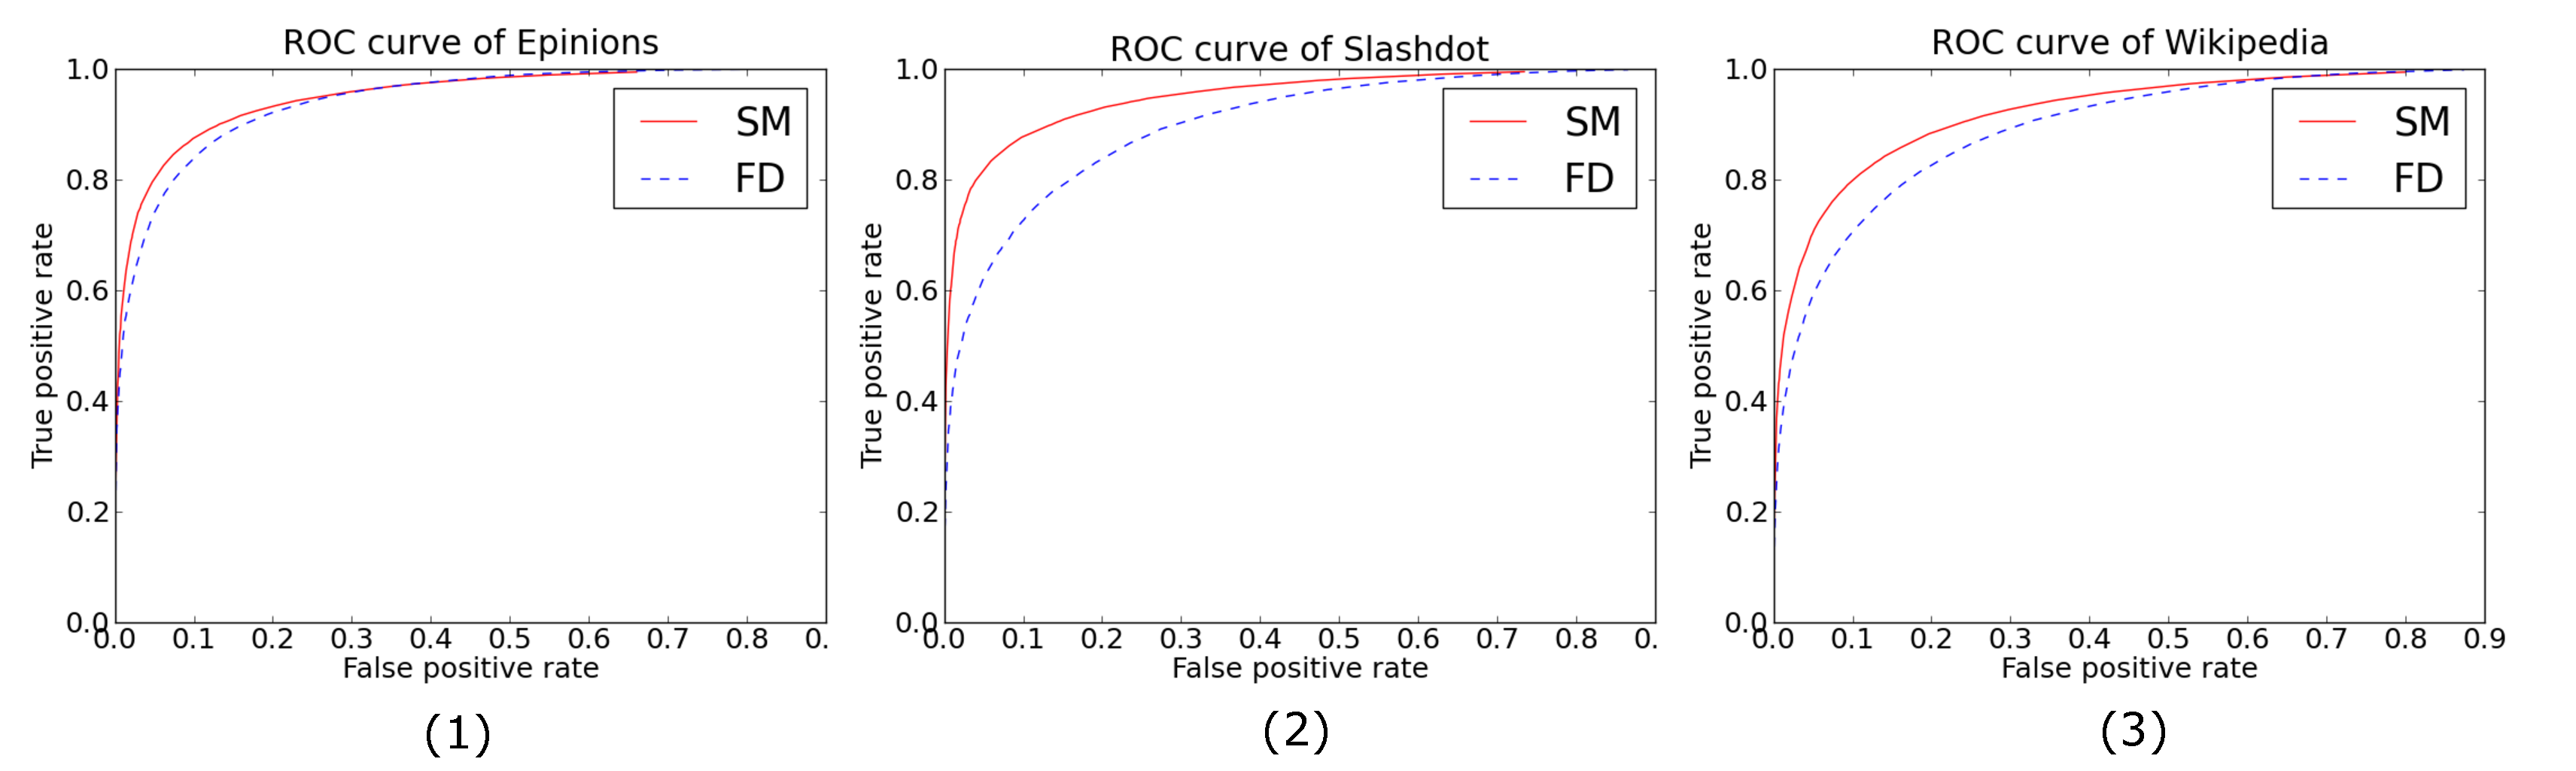
\includegraphics[height=1.8in]{Figs/ROC_curve.pdf}
\caption{\label{fig:ROC}The ROC curves are drawn upon
  distances of hidden edges, generated by SM and FD. (1) (2) (3)
  correspond to the ROC curves generated from Epinions, Slashdot and
  Wikipedia datasets respectively.}
\end{figure}

For all three datasets, we find the ROC curve of $SM$ is on the
``northwest'' side of the one of $FD$, which indicates SM is
consistently better than FD in separating hidden positive edges from
negative ones. Notice that the improvement for Slashdot is the most
significant one among the three. The possible explanation is in
Slashdot edges represent ``friends'' or ``foes'', which is by nature a
more clear identification of trust and distrust, whereas in votes in
Wikipedia or distrusting reviews of other users in Epinions are not as
strong distrust relations.  As a result, our convergence model
characterizes its mutual relation based structure nicely, and hence
produces good prediction performance.

On the Epinions and Slashdot datasets, the best thresholds on ROC
curve give $88-90 \%$ accuracy on both positive and negative
hidden edges. For Wikipedia, we achieves $83-85 \%$ at the best
threshold. The accuracy rates of Epinions and Wikipidea match the best
results from previous work, and the one of slashdot appears to be the
best so far.
\section{General Edge Prediction}
The {\it edge sign prediction} only
deals with the existing signed edges. In predicting the sign of a
hidden edge, we already know that the edge exists in the original
network. A more general problem is to predict whether there is positive edge between arbitrary pair of nodes~\cite{Kleinberg:03}. In theory, our convergence model should
be able to make such general predictions. The difference is that we do
not know if there is a hidden edge or not. We generate the distances of
testing edges as before. Now, instead of classifying the hidden edges
in $G_{r^{'}}$ as positive/negative, we need to classify them as positive or not.

The {\it general edge prediction}, deciding whether an positive edge exists or
not, is obviously a harder problem than {\it edge signed
  prediction}. Social networks are usually sparse, and hence there are
a lot more neutral relations than biased relations. If larger
distances represent more negativeness (less positiveness), then the
distance of a neutral relation should be smaller than a negative one
and larger than a positive one. As a consequence, the distribution of
neutral edges in terms of distance should concentrate in the middle
range distances. We next study this distribution, as a preliminary
step to solve the {\it general edge prediction} problem.

For each dataset, we generate samples based on random source nodes as
before, except that we exclude the edges between the $k$ source
nodes. Instead of cross validation, we use the entire sub-network for
training, and use the $k(k-1)/2$ edges between the $k$ source nodes as
testing data, whose signs are available in the original dataset
(positive, negative or neutral, i.e. no link). Similarly, the signs of
the testing edges should not be influenced strongly by the other edges
in the network. Hence, after convergence they should get to the
distances corresponding to their true signs. We repeat the experiments
50 times over all three datasets, and collect the distances for only
the neutral testing edges.
\begin{figure}[th]
\centering
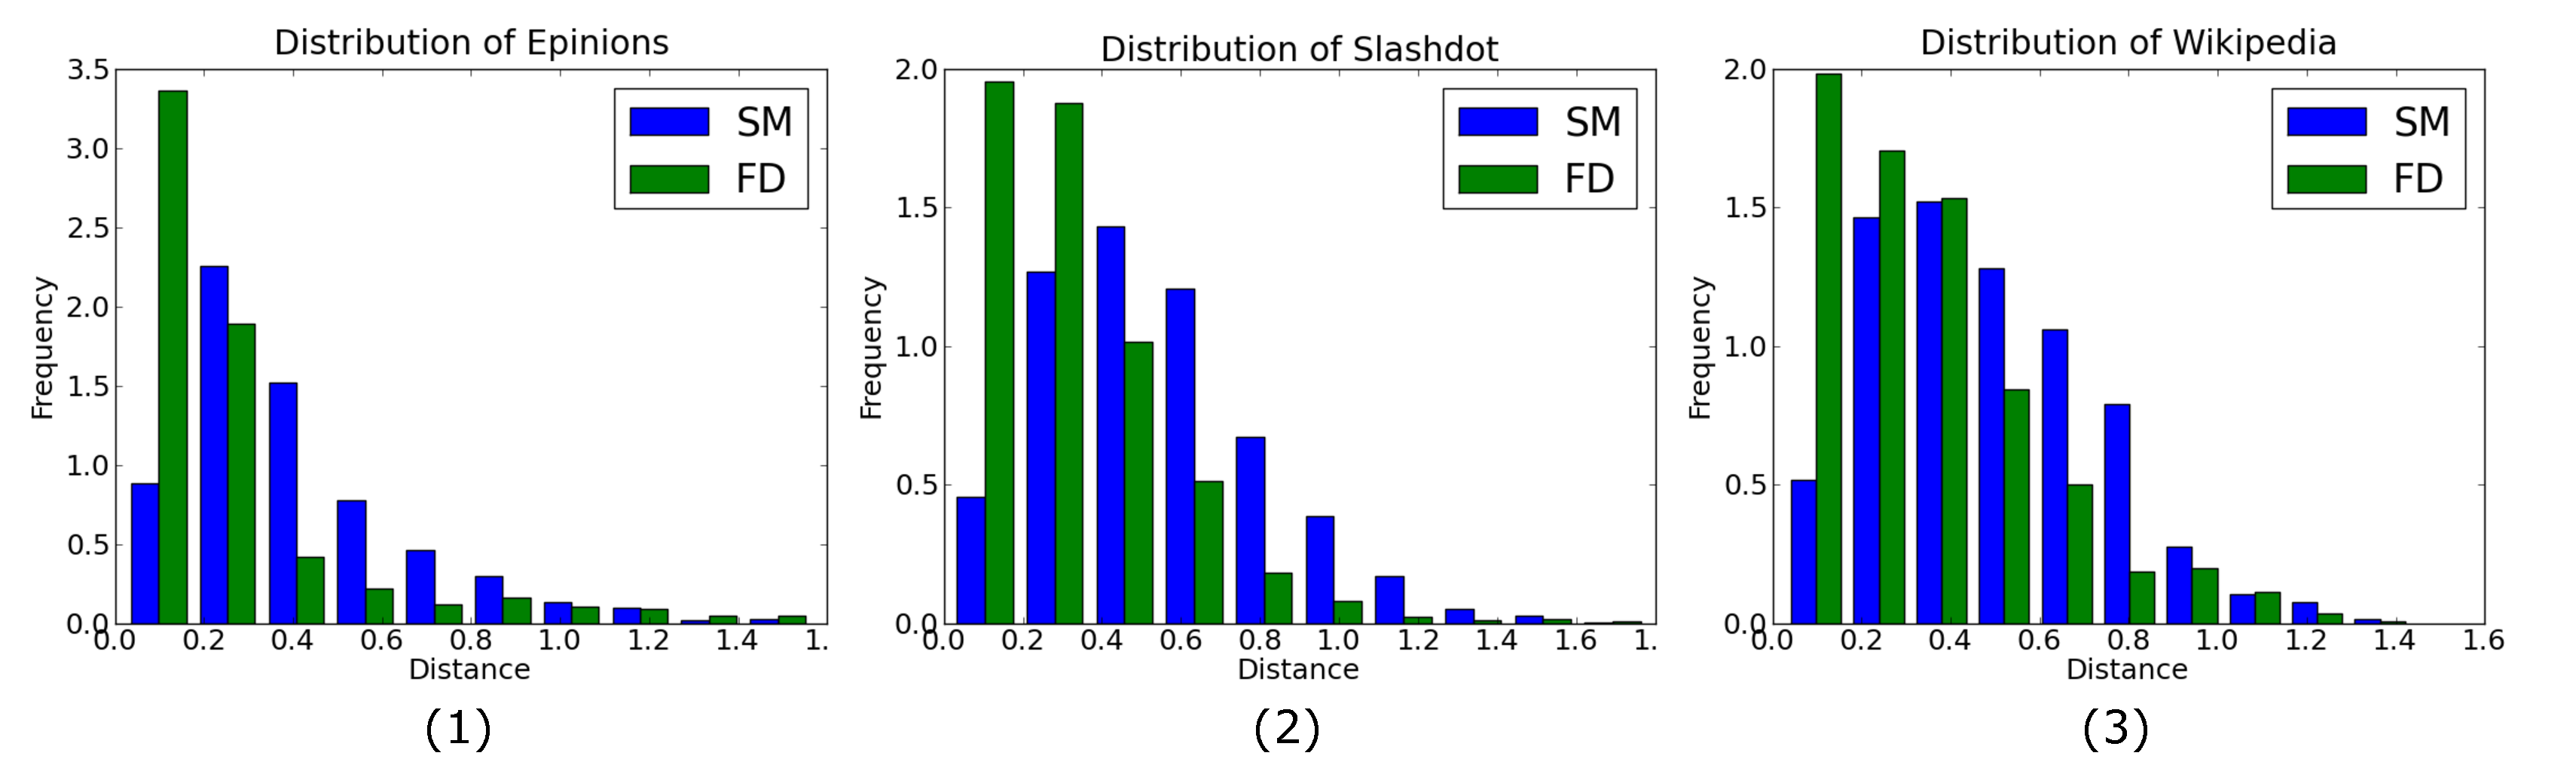
\includegraphics[height=1.8in]{Figs/hist1.pdf}
\caption{\label{hist}The histograms are drawn upon distances of
  neutral testing edges, generated by SM and FD. (1) (2) (3)
  correspond to the histograms generated from Epinions, Slashdot and
  Wikipedia datasets respectively.}
\end{figure}

As it is shown in Figure~\ref{hist}, the distances of neutral testing
edges generated by SM do relatively concentrate in the middle-range of
values following an almost Gaussian distribution. On the contrast, the
majority of neutral testing edges's distances by FD have small values,
implying a positive prediction. In fact, based on the distributions,
we can conclude that it is much more probable to classify a missing
link as a positive edge in FD than in SM.  However, SM provides more
flexibility as the distances are distributed over a larger range with
an almost Gaussian distribution, allowing us to test different tunable
algorithms.

The experimental results show the superiority of our convergence model
in predicting signed edges. Moreover, they justify that our general
balance theory is a relatively accurate description of the stable
state of social networks, and that the convergence model correctly
characterizes the dynamics of social network. As a result, our model
is a good starting point for developing algorithms for solving the
{\it general edge prediction} problem.


%Charpter of Conclusions
%%%%%%%%%%%%%%%%%%%%%%%%%%%%%%%%%%%%%%%%%%%%%%%%%%%%%%%%%%%%%%%%%%% 
%                                                                 %
%                            CHAPTER SEVEN                          %
%                                                                 %
%%%%%%%%%%%%%%%%%%%%%%%%%%%%%%%%%%%%%%%%%%%%%%%%%%%%%%%%%%%%%%%%%%% 
 
\chapter{CONCLUSIONS AND FUTURE WORK}
In this thesis, we introduced a general model for structural balance
theory that can handle relation strengths and generalizes the
classical balance theory. We showed that our notion of balance can be
mapped to triangular inequality over metric distances and the issue of
convergence can be modeled as the metric multidimensional scaling
problem for which stress majorization provides exact solutions. We
have shown that our theory can be used to effectively solve the edge
sign prediction problem and its performance matches and exceeds state
of the art for this problem. This is due to the fact that positive and
negative edges are mapped to a continuous range of strengths based on
the constraints provided by the other nodes. However, in contrast with
previous work, our method is aware of global constraints based on
balance which results in better results overall. Furthermore, the
solutions provided by our method can also be used to solve the harder
edge prediction problem.

We are investigating various avenues of future work. Inspired by the
work in~\cite{Khoury:12}, we have developed an approximation algorithm
of stress majorization in the context of social networks. We would like to implement and test how well the approximation is. Furthermore, we are currently testing how the inclusion of relation
strength improves performance by considering other actions of the
users that imply the existence of a social tie. Our method also has
applications to many related problems like clustering and link
prediction, which we are currently investigating. We are studying the
various properties of our theory in general networks and how it can be
extended to an asymmetric interpretation of links.  We note that our
method not only allows us to make predictions, but also study the
characteristics existing networks and compare various
characteristics. Example measures would be the ratio between positive
and negative distances or between largest and smallest
distances. These measures can help us develop new insights into the
nature of adversarial relationships in different networks.

%%%%%%%%%%%%%%%%%%%%%%%%%%%%%%%%%%%%%%%%%%%%%%%%%%%%%%%%%%%%%%%%%%%% 
%                                                                 %
%                           BIBLIOGRAPHY                          %
%                                                                 %
%%%%%%%%%%%%%%%%%%%%%%%%%%%%%%%%%%%%%%%%%%%%%%%%%%%%%%%%%%%%%%%%%%% 
 
%This method produces a numbered bibliography where the numbers
%correspond to the \cite commands in the text. See the LaTeX manual.
%
\specialhead{LITERATURE CITED}
\begin{singlespace}
\begin{thebibliography}{99}
\bibitem{thisbook} This is the first item in the Bibliography.
Let's make it very long so it takes more than one line.
Let's make it very long so it takes more than one line.
Let's make it very long so it takes more than one line.
Let's make it very long so it takes more than one line. 
\bibitem{anotherbook} The second item in the Bibliography.
\bibitem{yetanotherbook} Another item in the Bibliography.
\end{thebibliography}
\end{singlespace}
   
%This is an alternative method.  It's a simple unnumbered bibliography
%with hanging indentation.
%
\specialhead{BIBLIOGRAPHY}
\begin{singlespace}
\bibentry This is the first item in the Bibliography.
Let's make it very long so it takes more than one line.
Let's make it very long so it takes more than one line.
Let's make it very long so it takes more than one line.
Let's make it very long so it takes more than one line.
Let's make it very long so it takes more than one line. 
\bibentry The second item in the Bibliography.
\bibentry Another item in the Bibliography.
  
\end{singlespace} 

% This file was created with JabRef 2.5.
% Encoding: UTF-8

@incollection{Ames:2011,
author = "D.L. Ames and S.T. Fiske and A.T Todorov",
title = "Impression Formation: A Focus on Others’ Intents",
year = "2011",
booktitle = "The Oxford Handbook of Social Neuroscience",
editor = "J. Decety and J. Cacioppo",
publisher = "Oxford University Press",
pages = "419-433"
}

@ARTICLE{Fiske:2007,
title = "Universal dimensions of social cognition: warmth and competence",
journal = "Trends in Cognitive Sciences",
volume = "11",
number = "2",
pages = "77 - 83",
year = "2007",
note = "",
issn = "1364-6613",
doi = "10.1016/j.tics.2006.11.005",
url = "http://www.sciencedirect.com/science/article/pii/S1364661306003299",
author = "Susan T. Fiske and Amy J.C. Cuddy and Peter Glick"
}

@BOOK{Adali:2013,
  title = {Modeling Trust Context in Networks},
  publisher = {Springer Briefs},
  year = {2013},
  author = {Sibel Adal{\i}}
}

@ARTICLE{Cartwright:56,
  author = {D. Cartwright and F. Harary},
  title = {Structural balance: a generalization of Heider's theory},
  journal = {Psychological Review},
  year = {1956},
  volume = {63},
  pages = {277-293},
  number = {5}
}

@ARTICLE{Davis:67,
  author = {J. Davis},
  title = {Clustering and structural balance in graphs},
  journal = {Human Relations},
  year = {1967},
  pages = {181-187}
}

@ARTICLE{Doreian:02,
  author = {P. Doreian},
  title = {Event sequences as generators of social network evolution},
  journal = {Social Networks},
  year = {2002},
  volume = {24},
  pages = {93-119},
  owner = {qiany3},
  timestamp = {2013.03.01}
}

@INPROCEEDINGS{golbeck:distrust2011,
  author = {T. DuBois and J. Golbeck and A. Srinavasan},
  title = {Predicting Trust and Distrust in Social Networks},
  booktitle = {IEEE International Conference on Social Computing},
  year = {2011}
}

@INPROCEEDINGS{DuBois:2009,
  author = {T. DuBois and J. Golbeck and A. Srinivasan},
  title = {Rigorous probabilistic trust-inference with applications to clustering},
  booktitle = {Proceedings of the 2009 IEEE/WIC/ACM International Joint Conference
	on Web Intelligence and Intelligent Agent Technology},
  year = {2009},
  volume = {01},
  pages = {655–658},
  publisher = {IEEE Computer Society}
}

@BOOK{kleinberg-book,
  title = {Networks, Crowds, and Markets: Reasoning About a Highly Connected
	World},
  publisher = {Cambridge University Press},
  year = {2010},
  author = {David Easley and Jon Kleinberg}
}

@ARTICLE{Gansner:05,
  author = {E. R. Gansner and Y. Koren and S. North},
  title = {Graph Drawing by Stress Majorization},
  journal = {J. Pach (Ed.), Graph Drawing, Lecture Notes in Computer Science},
  year = {2005},
  volume = {3383},
  pages = {239-250},
  publisher = {Berlin/Heidelberg: Springer}
}

@ARTICLE{Granovetter:1973,
  author = {M. Granovetter},
  title = {The Strength of Weak Ties},
  journal = {American Journal of Sociology},
  year = {1973},
  volume = {78},
  pages = {1-22},
  issue = {6}
}

@INPROCEEDINGS{Guha:04,
  author = {R. Guha and R. Kumar and P. Raghavan and A. Tomkins},
  title = {Propagation of trust and distrust},
  booktitle = {Proceedings of the 13th international conference on World Wide Web.
	ACM},
  year = {2004},
  pages = {403--412}
}

@ARTICLE{Heider:46,
  author = {F. Heider},
  title = {Attitudes and cognitive organization},
  journal = {Journal of Psychology},
  year = {1946},
  pages = {107-12}
}

@INPROCEEDINGS{Khoury:12,
  author = {M. Khoury and Yifan Hu and Shankar Krishnan and Carlos Scheidegger},
  title = {Drawing Large Graphs by Low-Rank Stress Majorization},
  booktitle = {EuroVis},
  year = {2012}
}

@INPROCEEDINGS{Leskovec:2010,
  author = {J. Leskovec and D. Huttenlocher and J. Kleinberg},
  title = {Predicting positive and negative links in online social networks},
  booktitle = {Proceedings of the 19th International Conference on World Wide Web},
  year = {2010},
  pages = {641--650}
}

@INPROCEEDINGS{Kleinberg:03,
  author = {D. Liben-Nowell and J. Kleinberg},
  title = {The link prediction problem for social networks},
  booktitle = {International Conference on Information and Knowledge Management
	(CIKM)},
  year = {2003},
  pages = {556-559}
}

@ARTICLE{Tomasello:2005,
  author = {Tomasello,Michael and Carpenter,Malinda and Call,Josep and Behne,Tanya
	and Moll,Henrike},
  title = {Understanding and sharing intentions: The origins of cultural cognition},
  journal = {Behavioral and Brain Sciences},
  year = {2005},
  volume = {28},
  pages = {675-91; discussion 691-735},
  number = {5}
}

@ARTICLE{Uzzi:1996,
  author = {Brian Uzzi},
  title = {The sources and consequences of embeddedness for the economic performance
	of organizations: The network effect.},
  journal = {American sociological review},
  year = {1996},
  volume = {61},
  pages = {674-698},
  issue = {4}
}




% Note that, if you wish, you can use BibTeX to create your bibliography
% from a database. See section 5.6.2 of Memo RPI.110 for information. 
%%% Local Variables: 
%%% mode: latex
%%% TeX-master: t
%%% End: 



\specialhead{REFERENCES}
\bibliographystyle{IEEEtran}
\bibliography{rpireference}

%%%%%%%%%%%%%%%%%%%%%%%%%%%%%%%%%%%%%%%%%%%%%%%%%%%%%%%%%%%%%%%%%%%
%                                                                 %
%                            APPENDICES                           %
%                                                                 %
%%%%%%%%%%%%%%%%%%%%%%%%%%%%%%%%%%%%%%%%%%%%%%%%%%%%%%%%%%%%%%%%%%%

\appendix % This command is used only once!
%\addcontentsline{toc}{chapter}{APPENDICES} %toc entry or:
\addtocontents{toc}{\parindent0pt\vskip12pt APPENDICES} %toc entry, no page #
\chapter{}
Follow Gansner's description, we denote the d-dimensional location matrix as $X$~\cite{Gansner:05}. Let node $i$'s location be $X_{i}$. The stress function in literature is defined as
\begin{equation}\label{stress1}
stress(X)=\sum_{i<j} w_{ij} (||X_{i}-X_{j}|| - d_{ij})^{2}\,,
\end{equation}
where $w_{ij}$ are weights and $d_{ij}$ denote the ideal distance between $i$ and $j$. The MDS is an optimization problem to minimize the total stress. Equation~\ref{stress1} can be decomposed and we have
\begin{equation}\label{stress2}
stress(X)=\sum_{i<j} w_{ij}d_{ij}^{2} + \sum_{i<j}w_{ij}||X_{i}-X_{j}||^{2}- 2\sum_{i<j}w_{ij}d_{ij}||X_{i}-X_{j}||.
\end{equation}
The first term of~\ref{stress2} is a constant. The second term, $\sum_{i<j}w_{ij}||X_{i}-X_{j}||^{2}$, is a quadratic sum, and hence can be written as
\[ \sum_{i<j}w_{ij}||X_{i}-X_{j}||^{2} = Tr(X^{T}L^{w}X)\,, \]
where $L^{w}$ is a weighted matrix, defined as
\[
  L_{i,j}^{w}=\left\{ 
  \begin{array}{l l}
    -w_{ij} \quad & i \neq j\\
    \sum_{k \neq i}w_{ik} \quad &i=j 
  \end{array} \right. \text{ .}
\]
The third term, $\sum_{i<j}w_{ij}d_{ij}||X_{i}-X_{j}||$, need extra attention. By Cauchy-Schwartz inequality, 
\[
||X_{i}-X_{j}|| ||Z_{i}-Z_{j}|| \geq (X_{i}-X_{j})^{T} (X_{i} - Z_{j})
\]
with the equality when $Z=X$. Hence, we have the following bound of the third term.
\[
\sum_{i<j}w_{ij}d_{ij}||X_{i}-X_{j}|| \geq \sum_{i<j}w_{ij}d_{ij} (X_{i}-X_{j})^{T} (X_{i} - Z_{j}) / ||Z_{i}-Z_{j}||.
\]
Equivalently, the right side of the inequality can be rewritten in the trace form.
\[
\sum_{i<j}w_{ij}d_{ij} (X_{i}-X_{j})^{T} (X_{i} - Z_{j}) / ||Z_{i}-Z_{j}||=Tr(X^{T}L^{Z}X),
\]
where $L^{Z}$ is defined as
\[
  L_{i,j}^{Z}=\left\{ 
  \begin{array}{l l}
    -w_{ij}d_{ij}/||Z_{i}-Z_{j}|| \quad & i \neq j\\
    -\sum_{j \neq i}L_{i,j}^{Z} \quad &i=j 
  \end{array} \right. \text{ .}
\]
From the above all, we can bound the stress function confidently by function $F^{Z}(X)$, defined as
\begin{equation}
F^{Z}(X)=\sum_{i<j}w_{ij}d_{ij}^{2}+Tr(X^{T}L^{w}X)-2Tr(X^{T}L^{Z}Z)
\end{equation}
with equality when $Z=X$.
Notice $^{Z}(X)$ is of quadratic form, and we can easily find its minima by differentiate it by X and solve
\[
L^{w}X=L^{Z}Z.
\]
This leads to the following iterative optimization process. Given the location matrix at time $t$, $X(t)$, we want to compute $X(t+1)$ so that $stress(X(t+1)) < stress(X(t))$. We take $X(t+1)$ as the minimizer of $F^{X(t)}(X)$ by solving the above equation iteratively. At this point, if $X(t+1)=X(t)$, the process is terminated. Otherwise, we get
\[
stress(X(t+1)) \leq F^{X(t)}(X(t+1)) < F^{x(t)}(X(t)) =stress(X(t)).
\]
To summarize, the majorization process involves solving the following equation iteratively
\begin{equation}
L^{w}X(t+1)=L^{X(t)}X(t),
\end{equation}
where $L^{w}$ is constant throughout the process, whereas matrix $L^{X(t)}$ need to be computed at each iteration.
While stress majorization is an effective and accurate optimization strategy, it is not feasible in very large networks. Solving (14) in each iteration requires the computation of a fully dense matrix, which in total requires $O(n^3)$ time and $O(n^{2})$ space. For network of node number $> 10^{5}$, direct implementation of stress majorization becomes impossible.

\end{document}
